%This is the fourth chapter of the dissertation

%The following command starts your chapter. If you want different titles used in your ToC and at the top of the page throughout the chapter, you can specify those values here. Since Columbia doesn't want extra information in the headers and footers, the "Top of Page Title" value won't actually appear.

\pagestyle{cu}
\graphicspath{{./Chapter5/Figures/}}
\chapter[Purity and the Electron Lifetime][Purity and the Electron Lifetime]{Purity and the Electron Lifetime}
\label{chap:purification}

In a noble element dark matter detection experiment the purity of the target mass is an essential consideration and must be consistently
measured.  The effects of electronegative impurities - which attenuate light and charge - are easily measured through the electron
lifetime.  However, a reliable model for the evolution of the impurities does not exist to explain and predict the behavior.

This chapter focuses on the effects of impurities (\secref{sec:importance_procedure_effects}), electron lifetime measurements
(\secref{sec:electron_lifetime_measurements}), the derivation of the electron lifetime model (\secref{sec:electron_lifetime_model}), and
the results (\secref{sec:elifetime_fit}).



\section{Effects of Electronegative Impurities}
\label{sec:importance_procedure_effects}
Electronegative impurities mainly come from outgassing from detector materials.

Impurity usually refers to two distinct but correlated group, though the degree of the correlation can depend on the
experiment.  The first is background contamination from radioactive elements of other noble elements inside the TPC.  For xenon
the primary challenges are \ce{^{85}Kr} (\secref{subsubsec:backgrounds_electronic_krypton}) and \ce{^{222}Rn}
(\secref{subsubsec:backgrounds_electronic_radon}) as they have low-energy decays that can reach our region of interest.

The second type is the density of electronegative impurities such as \ce{O_2} or
\ce{N_2}, which attach to drifting electrons, lowering or even eliminating the S2.  This can have the largest impact at low energies
since the number of \electron is much fewer.  To correct for the expected initial number of electrons we can use the electron lifetime
$\tau_{\mathrm{e}}$.  Of course, if the entire cloud of electrons is
removed by these impurities we cannot apply a correction since we have no knowledge of where in the detector it occurred or the energy
deposition.  Even if some electrons make it to the surface a low electron lifetime creates more uncertainty when correcting the S2.  This
chapter is focused electronegative impurities, though its examination necessitates consideration of the radioactive background
concentration.

\subsection{Photon Attenuation}
\label{subsec:importance_procedure_effects_photons}
Xe scintillation (178 nm with ${\sim} 14\ \mathrm{nm}$ spectral FWHM) is absorbed by a number of electronegative impurities
\citeref{Watanabe1953a, Watanabe1953b}.  At concentrations of ppm or higher
the fraction of VUV photons that reach the PMTs can be considerably decreased - especially for large detectors where longer travel
distances are required.  The intensity drop due to photon attenuation is given by

\vspace{-10pt}

\begin{equation}
I(x) = I_0 e^{-x / \lambda_{\mathrm{att}}}
\end{equation}

\noindent where $I_0$ is initial intensity, $x$ is distance, and $\lambda_{\mathrm{att}}$ is the attenuation length, and
$1 / \lambda_{\mathrm{att}} = 1 / \lambda_{\mathrm{abs}} + 1 / \lambda_{\mathrm{scatt}}$ where $\lambda_{\mathrm{abs}}$ and
$\lambda_{\mathrm{scatt}}$ are the the absorption and scattering lengths, respectively.  The absorption length describes loss of
photons due to absorption by an element or molecule while the scattering length describes the elastic scattering of photons.  For
perfectly pure xenon
$\lambda_{\mathrm{abs}} \sim \infty$ (\citeref{Baldini2005} found $\lambda_{\mathrm{abs}} > 100\ \mathrm{cm}$ at 90\% confidence
level).

High levels of impurities, however, can shorten the absorption
length.  \figref{fig:importance_procedure_effects_photons_absorption_coefficents} shows the absorption coefficients
($\lambda_{\mathrm{abs}}^{-1}$) for 1 ppm \htwoo and \otwo from $130 \mdash 200\ \mathrm{nm}$.  They overlap with shorter wavelengths
of the xenon spectrum (included for comparison), meaning light detected by PMTs will have an asymmetric distribution.  With a nearly
1-meter tall detector a 1 ppm concentration of \htwoo would have at 10\% effect or more at ${\lesssim}\, 180\ \mathrm{nm}$.

\begin{figure}
\centering
\includegraphics[width=0.8\textwidth]{absorption_spectra}
\caption[Absorption coefficient for photons at 1 ppm \ce{H_2O} vapor and \ce{O_2}.  The Xe scintillation
spectrum is overlaid for comparison.]{Absorption coefficient for photons at 1 ppm \ce{H_2O} vapor (solid red) and \ce{O_2} (dashed green).  The Xe scintillation
spectrum is overlaid for comparison (dashed blue).  \ce{H_2O} impacts Xe scintillation considerably
more than \ce{O_2} when at the same concentration.  Image credit: \citeref{Ozone2005}, \ce{H_2O} data from \citeref{Yoshino1996}.}
\label{fig:importance_procedure_effects_photons_absorption_coefficents}
\end{figure}

The relative intensities for different \ce{H_2O}/Xe and \ce{O_2}/Xe concentrations from $0 \mdash 60\ \mathrm{cm}$ are shown in
\figref{fig:importance_procedure_effects_photons_absorption_distance}.  At the level of $\mathcal{O}(100)\ \mathrm{ppb}$ of
oxygen $I / I_0 > 0.8$ at 60 cm.  The effect of water is substantially worse with $I / I_0 < 0.3$, highlighting the need for
significant reduction LXe experiments.  Even with a LXe purity that is appreciably better than
\figref{fig:importance_procedure_effects_photons_absorption_distance} $\lambda_{\mathrm{att}} \approx \lambda_{\mathrm{abs}}$ since
the effects of scattering are subdominant with respect to absorption.

\begin{figure}
\centering
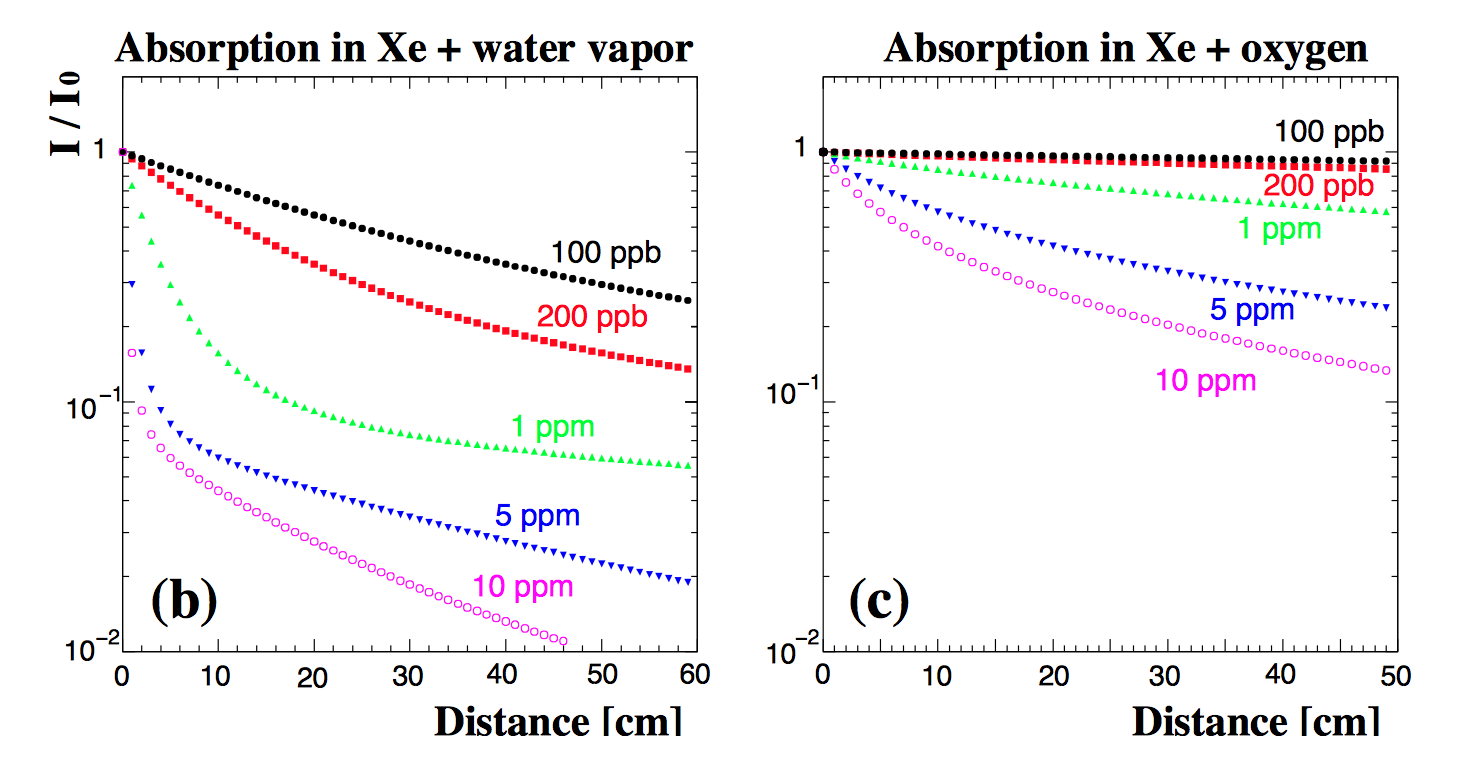
\includegraphics[width=\textwidth]{AbsorptionWithDistance}
\caption{Fraction of initial intensity of xenon scintillation with distance for various concentrations of \htwoo (left) and \otwo
(right).  Image credit: \citeref{Ozone2005}.}
\label{fig:importance_procedure_effects_photons_absorption_distance}
\end{figure}

Photon attenuation ultimately increases our energy threshold as we are less sensitive to lower energies as few photons are
measured.



\subsection{Charge Depletion}
\label{subsubsec:importance_procedure_effects_charge}
As the electron cloud following a recoil drifts it diffuses
longitudinally (in the direction of $E_{d}$) and transversely (perpendicular to $E_{d}$).  The
diffusion coefficients $D_{L}$ and $D_{T}$ depend on the electric field with $D_{T}/D_{L} \sim 10$.  The electron spread is
$\sigma_{D_{T}} = \sqrt{D_{T} t_{d}}$ where $t_{d} = d/v_{d}$ is the drift time and $d$ is the drift distance.

The behavior of electrons can be classified according to their mobility in the limit of $E \rightarrow 0$, $\mu_0$.  When LXe is
polarized by electrons its high polarizability ($4.0 \times 10^{-24}\ \mathrm{cm^3}$, highest for among noble gases) make it
attract \electron and interact with nearby Xe atoms through dipole-dipole interactions.  The equilibrium of these two effects
determines the potential energy of the ground state of electrons $V_0$, which is anti-correlated with $\mu_0$.  For LXe these have
been measured to be $V_0 = -0.61 \pm 0.05\ \mathrm{K}$ \citeref{Tauchert1977} and $\mu_0 = 2200 \pm 200\ \mathrm{cm^2\ V^{-1}\ s^{-1}}$
\citeref{Yoshino1976} at $165\ \mathrm{K}$ (in addition $\mu_0$ was found to be $1900$ and $2200\ \mathrm{cm^2\ V^{-1}\ s^{-1}}$
at $163\ \mathrm{K}$ by \citeref{Yoshino1976} and \citeref{Miller1968}, respectively).  The large electron mobilities indicate the
electrons are \textit{quasifree}, and have drift velocities that can exceed even those of GXe, as shown in
\figref{fig:importance_procedure_effects_charge_drift_velocity}.

\begin{figure}
\centering
\includegraphics[width=0.8\textwidth]{drift_velocity_field}
\caption[Drift velocity (here defined as $W$) dependence on reduced electric field $E_d/N$ where $N$ is the number of molecules per
volume.]{Drift velocity (here defined as $W$) dependence on reduced electric field $E_d/N$ where $N$ is the number of molecules per
volume.  Points are from experimental data \citeref{Gushchin1982, Huang1978, Wagner1967, Pack1992} and curves are from
calculations.  $1\ \mathrm{Td} = 10^{-17}\ \mathrm{V\ cm^2}$.  LXe has a higher drift velocity than GXe at
$E_d/N \lesssim 1\ \mathrm{Td}\ (1\ \mathrm{Td} = 10^{-17}\ \mathrm{V\ cm^2})$.  Image credit: \citeref{Atrazhev2005}.}
\label{fig:importance_procedure_effects_charge_drift_velocity}
\end{figure}

Ions exhibit significantly lower mobility than electrons.  Their mobilities are parameterized as $\mu \approx \eta^{-\alpha}$ where
$\eta$ is the liquid viscosity and $\alpha = 1 \mdash 2$.  The diffusion coefficients can be calculated with the Nernst-Einstein equation

\vspace{-10pt}

\begin{equation}
\frac{e D(E)}{\mu (E)} = \mathcal{F} \langle E \rangle
\end{equation}

\noindent where $\mathcal{F} = 0.5 \mdash 1$ depends on the electron distribution function (e.g. $\mathcal{F} = 2/3$ for a
Maxwellian distribution).

The mobilities for holes, \ce{TMSi^+}, \ce{O_2^-}, \ce{^{226}Th}, \ce{^{208}Tl}, and \ce{Xe_2^+} in in LXe are listed in
\tabref{tab:importance_procedure_effects_charge_mobilities}.  They are ${\sim} 10^6$ times smaller than the electron mobility.

\begin{table}
\centering
\begin{tabular}{cccccc}
\hline
\hline
Ion & T [K] & $\mu\ [10^{-4}\ \mathrm{cm^2\ V^{-1}\ s^{-1}}]$ & Ref. \\
\hline
holes & 161 & 35 & \citeref{Hilt1994b} \\
holes & 230 & 46 & \citeref{Hilt1994b} \\
\ce{TMSi^+} & 162 & 2 & \citeref{Hilt1994a} \\
\ce{TMSi^+} & 192 & 3 & \citeref{Hilt1994a} \\
\ce{O_2^-} & 162 & 6 & \citeref{Hilt1994a} \\
\ce{O_2^-} & 192 & 10 & \citeref{Hilt1994a} \\
\ce{^{226}Th^+} & 162 & 2.4 & \citeref{Wamba2005} \\
\ce{^{208}Tl^+} & 163 & 1.33 & \citeref{Walters2003} \\
\ce{Xe_2^+} & 184.2 & 2.85 & \citeref{Davis1962} \\
\ce{Xe_2^+} & 192.1 & 3.17 & \citeref{Davis1962} \\
\hline
\hline
\end{tabular}
\caption{Ion mobilities in LXe.  All ions listed are positive with the exception of \ce{O_2^-}.  Positive holes have mobilities that are
${\sim} 10$ times larger than ions.  Summarized data is given in \citeref{Aprile2006a}.}
\label{tab:importance_procedure_effects_charge_mobilities}
\end{table}

Hole mobility can be described by the hopping model of charge carrier transport.  In this temperature-dependent model charge is
propagated through jumps between traps yielding

\vspace{-10pt}

\begin{equation}
\mu = \frac{e b^2}{k_{\mathrm{B}} T} \omega
\label{eq:importance_procedure_effects_charge_mobility_simple}
\end{equation}

\noindent where $b$ is the average jump distance and $\omega$ is the jumping frequency, parameterized as

\vspace{-20pt}

\begin{equation}
\omega = P \Big( \frac{\omega_0}{2 \pi} \Big) e^{-E_{\mathrm{a}} / k_{\mathrm{B}} T}
\end{equation}

\noindent where $\omega_0$ is the phonon frequency and $P(\omega_0 / 2 \pi)$ is the tunneling probability between adjacent holes with
activation energy $E_{\mathrm{a}}$.  \figref{fig:importance_procedure_effects_charge_hole_mobility} shows hole mobility in
LXe.  The solid curve represents a model that parameterizes \eqnref{eq:importance_procedure_effects_charge_mobility_simple} as

\vspace{-15pt}

\begin{equation}
b^3(T) = \sqrt{2} M / \rho (T)
\end{equation}

\noindent where $M$ is the atomic mass of xenon and $\rho (T)$ is the temperature-dependent density \citeref{Hilt1994b}.  It
additionally assumes the hole is self-trapped between two rare atoms in a potential well, forming a polaron.  It gives a hole mobility of

\vspace{-5pt}

\begin{equation}
\mu (T) = \frac{e b^2 (T)}{k_{\mathrm{B}}} \frac{2 \pi}{h} \sqrt{\frac{\pi}{4 E_a k_{\mathrm{B}} T}} J_0^2
e^{-2 \alpha b(T)} e^{-E_a / k_{\mathrm{B}} T}
\label{eq:importance_procedure_effects_charge_mobility_polaron}
\end{equation}

\noindent where $h$ is Planck's constant and and $J(T) = J_0 e^{-\alpha b(t)}$ is the transfer integral.

\begin{figure}
\centering
\includegraphics[width=0.8\textwidth]{hole_mobility}
\caption{Temperature-dependent drift mobility for holes in LXe.  Data is shown as empty triangles.  A fit
using \eqnref{eq:importance_procedure_effects_charge_mobility_polaron} is shown as the solid line.  Image credit: \citeref{Aprile2006a}
(redrawn from \citeref{Hilt1994b}).}
\label{fig:importance_procedure_effects_charge_hole_mobility}
\end{figure}

As the electron cloud drifts electronegative impurities bond to \electron

\vspace{-10pt}

\begin{equation}
e^{-} + S \rightarrow S^{-}
\label{eq:impurity_attach}
\end{equation}

\noindent where $S$ refers to the impurity (e.g. $e^- + \mathrm{O_2} \rightarrow \mathrm{O_2^-}$).

\begin{enumerate}
\item Radiative attachment is given by
\vspace{-10pt}
\begin{equation}
e^- + XY \rightarrow XY^- + h \nu
\end{equation}

\vspace{-10pt}

\noindent where $XY$ is some atom or molecule.

\item Dissociative electron attachment (DEA) is when a low-energy electron bonds to a molecule causing it to fracture.  The process
is given by

\vspace{-10pt}

\begin{equation}
\begin{aligned}
e^- + XY \rightarrow XY^* + e^- \rightarrow X^+ + Y^- + e^- \\
e^- + XY \rightarrow XY^- \rightarrow X + Y^-
\end{aligned}
\end{equation}

\noindent where molecule $XY$ is separated into components $X$ and $Y$.  \ce{O_2} has 5.116 eV dissociation energy (the energy needed to
separate the oxygen) and \ce{O^-} has electron affinity (energy released in forming ion) of 1.461 eV.

\item Three-body attachment proceeds via the two-stage Bloch-Bradbury reaction \citeref{Bloch1935, Herzenberg1969}

\vspace{-15pt}

\begin{equation}
\begin{aligned}
e^- + XY &\leftrightarrow (XY^-)* \\
(XY^-)^* + Z &\rightarrow XY^- + Z
\end{aligned}
\end{equation}

\noindent where $Z$ is an atom or molecule from the majority gas population.  It carries out the bonding energy between the
\electron and electronegative $XY$.  Oxygen was studied \citeref{Aleksandrov1993, Aleksandrov1981, Aleksandrov2009}.
\end{enumerate}



\section{Measuring the Electron Lifetime}
\label{sec:electron_lifetime_measurements}
Mono-energetic radioactive decays are used to measure the electron lifetime.  For XENON1T electron lifetimes were calculated
using elements distributed in the xenon, since external \gammaray sources such as \ce{^{137}Cs} and
wall events could not reach the FV.  This was done primarily with $\mathrm{^{83m}Kr}$, $\mathrm{^{129m}Xe}$, $\mathrm{^{131m}Xe}$,
\ce{^{212}Bi}, \ce{^{218}Po}, and \ce{^{222}Rn} (other lines such as the $39.6\ \mathrm{keV}$ of $\mathrm{^{129}Xe}$ and
$80.2\ \mathrm{keV}$ of $\mathrm{^{131}Xe}$ during nuclear recoil calibrations were used but the short half-lifes made measurements
difficult).  Information for each element is listed in \tabref{tab:electron_lifetimes_isotopes}.  An
additional method of minimizing the \stwob width of the
\ce{^{212}Pb} electronic recoil band to address a discrepancy between
$\mathrm{^{83m}Kr}$ and \alphadecays (\secref{subsec:electron_lifetimes_rn222_vs_kr83m}) was tried but the uncertainty was too large to
draw any conclusions.



\subsection{S2/S1}
\label{subsec:electron_lifetimes_measurement_ss}
In the period immediately following XENON1T coming online the electron lifetime was ${\sim} 0$ since purification began at roughly
the same time.  The first in-situ calibration was not performed until almost three months later and mono-energetic
background decays had not yet been investigated, though \ce{^{222}Rn} and \ce{^{218}Po} would have had too few events in the top of the
detector to be reliable anyways.  However,
S2/S1 - though not energy-independent - was enough so to give reasonable estimates.  It was too early to have official cuts but
the ones used were sufficient and based on a history of knowledge of TPC detectors.

S1 (S2) single scatter cuts required that the second largest S1 (S2) be ${<}\, 0.2$ that of the first.  The purpose of these cuts was to
prevent S1-S2 mismatching: the S1 cut would
remove the possibility that we do not observe the S2 of a scatter deep in the TPC, while the S2 eliminated any ambiguity in matching a
single S1 with two potential S2s.

To reject noise at least three PMTs were required to observe the S1.  This is the same cut that was used in the dark matter
analysis.  Finally, the fraction of light seen on the top PMT array must fall between $0.2 \mdash 0.6$ for S1s and $0.5 \mdash 0.9$ for
S2s.

On a few occasions a \ce{^{137}Cs} was placed outside the detector.  While the water and LXe self-shielding limited the fraction of
radiation that made it inside the TPC, there were enough events for measurements.  This method was used until early August 2016.

\begin{table}
\centering
\begin{tabular}{rccrcc}
\hline
\hline
Isotope & Decay & Energy & $t_{1/2}$ & Section & Notes \\
\hline
$\mathrm{^{83m}Kr}$ & IC & $32.2\ \mathrm{keV}$ & 1.83 h & \secref{subsec:electron_lifetimes_measurement_kr} & Calibration \\
$\mathrm{^{129m}Xe}$ & $\gamma$ & $236.2\ \mathrm{keV}$ & 8.88 d & \secref{subsec:electron_lifetimes_measurement_gammas} & Background following NR cal. \\
$\mathrm{^{131m}Xe}$ & $\gamma$ & $163.9\ \mathrm{keV}$ & 11.93 d & \secref{subsec:electron_lifetimes_measurement_gammas} & Background following NR cal. \\
\ce{^{212}Bi} & $\alpha$ & $6.207\ \mathrm{MeV}$ & 60.55 m & \secref{subsec:electron_lifetimes_measurement_alphas} & \ce{^{220}Rn} calibration \\
\ce{^{218}Po} & $\alpha$ & $6.115\ \mathrm{MeV}$ & 3.10 m & \secref{subsec:electron_lifetimes_measurement_alphas} & Background \\
\ce{^{222}Rn} & $\alpha$ & $5.590\ \mathrm{MeV}$ & 3.82 d & \secref{subsec:electron_lifetimes_measurement_alphas} & Background \\
\hline
\hline
\end{tabular}
\caption{Isotopes used for electron lifetime analysis.  Background \ce{^{222}Rn} and \ce{^{218}Po} \alphadecays allow continual
monitoring but have relatively low statistics.  $\mathrm{^{83m}Kr}$ and \ce{^{212}Bi} have high statistics but are only available during
calibrations.  Excited nuclear states $\mathrm{^{131m}Xe}$ and $\mathrm{^{129m}Xe}$ are present in background after nuclear recoil
calibrations but their half-lifes limit their viability after several weeks.}
\label{tab:electron_lifetimes_isotopes}
\end{table}



\subsection[$\alpha$-decays][$\alpha$-decays]{$\mathbf{\alpha}$-decays}
\label{subsec:electron_lifetimes_measurement_alphas}
The high energy and substantial stopping power (\figref{fig:mass_stopping_power}) of $\alpha$ interactions causes a large fraction of
electrons to recombine with their parent or nearby \ce{Xe^+} atoms.  Their S1s are significantly higher than electronic or nuclear recoils
so are
easily distinguishable.  Because they are so recognizable and do not scatter many of the cuts developed for the science run analysis are
not necessary (some may not be reliable since they were developed using low-energy electronic recoils).  Therefore, just a small
number of cuts are used.

Events must have $r_{\mathrm{rec}} < 36.94\ \mathrm{cm}$.  This is in part for consistency with the First Results FV
\citeref{Aprile2017f}, but also because the greatest inhomogeneities in the electric field are expected to be largest at the top,
bottom, and
sides of the TPC as seen in \figref{fig:xenon1t_tpc_efield}.  Changes in field will produce different light and charge yields
(\secref{subsec:det_char_ly_cy}), so the number of photons and electrons would vary according to position.  In addition, the impurity
attachment rate dependence on field will cause the rate of electron removal to change inside the TPC
(\secref{subsec:electron_lifetime_model_field}).  Finally, the radial cut removes \alphadecays near the wall that would lose drifting
\electron to the PTFE.

The fraction of light seen by the top PMTs from electroluminescence is tightly constrained by stable detector conditions
(\eqnref{eq:electronlum}).  The percentage of events that fail this cut is small but it is important to remove any
``fake'' or gas events (a cut on the S1 fraction seen by the top PMTs will also remove GXe events).

In addition data acquisition quality cuts are used in data selection.  The first is the high energy veto, which is triggered by a very
large S2.  The second is produced by one or more digitizers nearly filling its memory buffer, and is called a busy veto.  The third is
a busy type check, which removes events that have a busy signal anywhere in the waveform.  The final is an end of run check, which
disqualifies the last 21 seconds per run (each run is 1 hour).  Details for each are given in \secref{subsec:xenon1t_daq}.

\figref{fig:electron_lifetimes_measurement_alphas_s1} shows cS1 dependence on $z$ for the \alphadecays of \ce{^{222}Rn}
(${\sim} 5.1 \times 10^4 \ \mathrm{PE}$) and \ce{^{218}Po} (${\sim} 5.6 \times 10^4\ \mathrm{PE}$) after these cuts.  The large
S1s from events deep in the detector saturate PMTs in the bottom array, which leads to under-corrected cS1s as shown in the left
panel.  To correct for this the data are split into slices in $z$ and fit in cS1 with gaussians.  Fits in the region
$-40 \lesssim z \lesssim -10\ \mathrm{cm}$, where saturation is not present, are used to define the correct cS1 distribution, which is
extrapolated across the entire length of
the TPC.  Differences in fit parameters are used to relocate events deeper in the detector into the proper cS1 band.  The
$\alpha$-corrected cS1 distribution is shown in the right panel of \figref{fig:electron_lifetimes_measurement_alphas_s1}.

\begin{figure}
\centering
\includegraphics[width=\textwidth]{rn_po_cs1_alpha}
\caption[cS1 (left) and $\alpha$-corrected cS1 (right) dependence on $z$ for \ce{^{222}Rn} and \ce{^{218}Po} $\alpha$-decays.]{cS1 (left) and
$\alpha$-corrected cS1 (right) dependence on $z$.  The large \alphadecay S1s deep in
the TPC sature the bottom PMTs, causing an under-corrected cS1, which
results in the distortion seen in the left panel.  Near the top ($z \gtrsim -5\ \mathrm{cm}$) a similar effect is observed from top PMT
saturation.  The distortion is corrected in the right panel where the effect is much less significant.  The red and blue boxes highlight
the events selected to calculate $\tau_e$.  The colors of data markers correspond to $\mathrm{S2_b}$.}
\label{fig:electron_lifetimes_measurement_alphas_s1}
\end{figure}

Even with the $\alpha$-corrected cS1s there is saturation near the very bottom of the TPC.  The saturation is so great
here that events from \ce{^{222}Rn} and \ce{^{218}Po} cannot be distinguished from one another.  This is generally not a problem since it
lays outside the fiducial volume.  There is also some distortion at $z \gtrsim -5\ \mathrm{cm}$ from events
near the LXe surface, whose light is tightly concentrated in the top PMT array.

Selected \ce{^{222}Rn} and \ce{^{218}Po} events are indicated by red and blue boxes, respectively.  Events with $-89< z < -9\ \mathrm{cm}$
and $4.9 \times 10^4 < \alpha \mdash \mathrm{corrected\ cS1} < 5.3 \times 10^4\ \mathrm{PE}$ (\ce{^{222}Rn}) and
$5.35 \times 10^4 < \alpha \mdash \mathrm{corrected\ cS1} < 5.8 \times 10^4\ \mathrm{PE}$ (\ce{^{218}Po}) are used.  The electron
lifetimes are calculated independently, which provides a nice cross-check.  Because the decay of \ce{^{222}Rn} can leave \ce{^{218}Po}
in a charged state it has slightly fewer ($5 \mdash 10\%$) events.  Electron lifetimes are calculated using 48 hours of data in order to
get sufficient statistics.

The data is binned in drift time slices $\Delta t_d$ and an initial fit is performed on the 50th percentiles of the \stwob distributions
from each slice.  The purpose of this preliminary electron lifetime $\tau_e^{(\mathrm{p})}$ is to remove events that are far from the
distribution.  The data
in each $\Delta t_d$ slice is binned in cS1 and fit with a gaussian.  The means and standard deviations are then fit
with an exponential to give the final electron lifetime $\tau_e$.  An example can be seen in
\figref{fig:electron_lifetimes_measurement_alphas_elifetime}.  The pink dashed lines define the boundaries above and below which
events were cut using the preliminary fit.  \ce{^{222}Rn} (left) and \ce{^{218}Po} (right) have good agreement.

\begin{figure}
\centering
\includegraphics[width=\textwidth]{rn_po_electron_lifetime_log}
\caption[Electron lifetime measurements using \ce{^{222}Rn} (left) and \ce{^{218}Po} (right) from October 29-31, 2017.]{Electron lifetime
measurements using \ce{^{222}Rn} (left) and \ce{^{218}Po} (right) from October 29-31, 2017.  The red and blue
lines correspond to \ce{^{222}Rn} and \ce{^{218}Po}, respectively, and are drawn in the drift time region that was used for the fit (see
text for event selection).  They are each drawn in both panels to show the \stwob overlap, highlighting the need for the
$\alpha$-corrected cS1 cut.  The pink dashed lines mark the boundaries derived from the preliminary fit outside of which events were not
considered for the final fit.  The electron lifetime measurements agree within uncertainty.}
\label{fig:electron_lifetimes_measurement_alphas_elifetime}
\end{figure}

In \figref{fig:electron_lifetimes_measurement_alphas_elifetime} the results of both fits are plotted in each panel for comparison.  It is
clear that without the $\alpha$-corrected cS1 cut the overlap in \stwob would make it impossible to decouple the \ce{^{222}Rn} from
\ce{^{218}Po} events.  Originally a cS1 $\alpha$-correction map did not exist so \ce{^{222}Rn} and \ce{^{218}Po} were fit together.  This
turned out to give slightly lower electron lifetimes than independent fits.  Once
the $\alpha$-correction was developed $tau_e$ was re-computed; however, this was not possible for some of the pre-SR0 data that had been
deleted.

This method can in principle be used for any $\alpha$-emitting element distributed throughout the FV of the detector and is done so
for \ce{^{212}Bi} during \ce{^{220}Rn} calibrations.  Despite \ce{^{220}Rn} and \ce{^{216}Po} also being $\alpha$-emitters their short
half-lifes (55.6 s and 145 ms, respectively) exclude them from consideration.  \ce{^{220}Rn} and \ce{^{216}Po} are also $\alpha$-emitters
and are visible when the source valve is open.  However, between the requirement that the source valve be closed and the time it takes to
see
the rate stabilize and switch to good data taking their short half-lifes (55.6 s and 145 ms, respectively) exclude them from
observation.  Even if this were not the case the $\alpha$-corrected cS1s of \ce{^{220}Rn} (6.405 MeV) and \ce{^{212}Bi} (6.207 MeV)
overlap, so a joint
measurement is likely to lead to a biased $\tau_e$.  Due to the enormous number of events there is also some small overlap between
\ce{^{220}Rn} and \ce{^{216}Po} (6.906 MeV).



\subsection[$\mathrm{^{83m}Kr}$][$\mathrm{^{83m}Kr}$]{$\mathbf{^{83m}Kr}$}
\label{subsec:electron_lifetimes_measurement_kr}
\ce{^{83}Rb} electron capture produces \metakr with a 74.8\% branching ratio.  The delayed coincidence between the 32.2 and 9.4 keV
conversion electrons differentiate $\mathrm{^{83m}Kr}$ from background.  With
$t_{1/2} = 154.4\ \mathrm{ns}$ for the 9.4 keV a large fraction of the S1s will overlap.  To select events that should always have
distinguishable S1s a cut requires
the time between S1s $\Delta t_{\mathrm{S1}}$ to be between 500 and 2000 ns (${<}\, 3 \times 10^{-4}\%$ of events have
$\Delta t_{\mathrm{S1}} > 2000\ \mathrm{ns}$).  This cut eliminates more than 96\% of \metakr events, but the remaining events are high
enough that $\tau_e$ measurements (and other studies, \secref{sec:det_char}) can be done.  To avoid PMT noise coincidence that might mimic
the 9.4 keV S1
the number of PMTs that see the low-energy peak must be $\geq 3$.  However, to ensure the coincidence is from \metakr events it is also
required to be $\leq 30$.

The S1 and S2 from each decay are matched by size of signal.  With such a short half-life $z$ cannot change much between decays so
$\tau_e$ does not have an important role at this stage.  Once the position coordinates are calculated from the S2 the S1s are
corrected.  The left panel of \figref{fig:electron_lifetimes_measurement_kr_cs1_halflife} shows the cS1s for both peaks inside the
1 t FV.  From the
almost entirely empty background it is clear how effective the $\Delta t_{\mathrm{S1}}$ cut is.  The number of events vs.
$\Delta t_{\mathrm{S1}}$ is shown in the right panel.  A fit to an exponential gives $t_{1/2} = 158 \pm 12.6\ \mathrm{ns}$, which
agrees with the accepted value.

\begin{figure}
\centering
\includegraphics[width=\textwidth]{kr_cs1_a_cs1_b_halflife}
\caption[cS1s for \metakr during final Science Run 1 calibration (left) and S1 delay time cut dependence of events from
$500 \mdash 2000\ \mathrm{ns}$.]{cS1s for \metakr during final Science Run 1 calibration (left).  The S1 delay time cut is remarkably efficient at selecting
\metakr and rejecting background.  S1 delay time cut dependence of events from $500 \mdash 2000\ \mathrm{ns}$ (right).  A fit with
an exponential gives a half-life of $158 \pm 12.6\ \mathrm{ns}$, which is in agreement with the accepted value of 154.4 ns.}
\label{fig:electron_lifetimes_measurement_kr_cs1_halflife}
\end{figure}

The electron lifetime is calculated using the 32.2 keV decay with a procedure similar to that of \alphadecays
\secref{subsec:electron_lifetimes_measurement_alphas}.  An preliminary fit is performed using the median \stwob in each drift time
slice.  However, the high statistics and near-total background removal by the $\Delta t_{\mathrm{S1}}$ cut
removes the need to exclude events far from the true \metakr (events farther than pink dashed lines in
\figref{fig:electron_lifetimes_measurement_alphas_elifetime}).  Each slice in drift time is fit with a gaussian, and an exponential
is fit to the results.

\begin{figure}
\centering
\includegraphics[width=0.9\textwidth]{kr_electron_lifetime_log}
\caption{Electron lifetime measurement using \metakr from January 23-25, 2018.}
\label{fig:electron_lifetimes_measurement_kr_elifetime}
\end{figure}

The large statistics provide $\tau_e$ measurements with precision that is only rivaled by \ce{^{212}Bi}.  Unfortunately, unlike
\alphadecays there are no other electronic recoil $\tau_e$ measurements performed regularly to corroborate these results, aside from
$\mathrm{^{129m}Xe}$ and $\mathrm{^{131m}Xe}$ following \ambe and NG calibrations.  \secref{subsec:electron_lifetimes_rn222_vs_kr83m}
discusses the reason for the discrepancy between \alphadecays and \metakr and which to use when correcting data.



\subsection{$\mathbf{\gamma}$-rays}
\label{subsec:electron_lifetimes_measurement_gammas}
The full absorption peak of \gammarays make them great candidates for electron lifetime measurements.  Unfortunately nearly all
\gammarays in the TPC come from elements in detector materials or external sources placed inside the water tank
(e.g. \ce{^{137}Cs}).  However, nuclear recoils can excite \ce{^{129}Xe} and \ce{^{131}Xe} nuclei to metastable states with half-lifes
of 8.88 and 11.93 days, respectively.  These metastable states serve as an in-situ calibration that are used to measure a number of
detector parameters including light and charge yield (\secref{subsec:det_char_ly_cy}), $g_1/g_{2\mathrm{b}}$
(\secref{subsec:det_char_photon_charge_efficiencies}), and electron lifetime.  While these evaluations can validate
electronic recoil measurements from \meta{83m}{Kr}, their short half-lifes limit them to the few weeks following an \ambe or NG
calibration.

Selecting $\mathrm{^{129m}Xe}$ and $\mathrm{^{131m}Xe}$ events is trickier than $\alpha$ or \meta{83}{Kr}.  This is in part because they
sit
on top of an ER background (see \figref{fig:calibrations_photon_charge_efficiences_ces_resolution} for background energy spectrum), have a
relatively low event rate, and do not have properties that allow a high-percentage cut
efficiency (e.g. \meta{83}{Kr} delayed coincidence or high \alphadecay S1).  Instead a number of cuts are required
to remove unwanted data before the fit.

\begin{figure}
\centering
\includegraphics[width=0.8\textwidth]{xe_meta_cs1_cs2b_sr1}
\caption{cS1 vs. \cstwob for $r_{\mathrm{rec}} < 36.94\ \mathrm{cm}$, $-6 < z < -85\ \mathrm{cm}$ for dark matter search data from April
1-7, 2017 following the SR1 \ambe calibration.  $\mathrm{^{129m}Xe}$ and
$\mathrm{^{131m}Xe}$ photopeaks are fit with a 2-dimensional gaussian to reject other background.  The red contours mark
the $4\sigma$ lines.}
\label{fig:electron_lifetimes_measurement_gammas_cs1_cs2}
\end{figure}

To select the 163.9 and 236.2 keV peaks an S2 single scatter cut (same as in nuclear recoil band fitting,
\secref{subsec:er_nr_calibrations_parameter_determ_cuts}) is used to remove much of the underlying background.  Additional data quality
cuts include ensuring the fraction of the S2 seen by the top PMTs and the width of the S2 fall within expected distributions.  For the FV
the usual $r_{\mathrm{rec}} < 36.94\ \mathrm{cm}$ is applied but we require $-85 < z < -10\ \mathrm{cm}$ to remove \gammarays of the same
energy from materials that penetrate deeper into the detector.

\begin{figure}
\centering
\includegraphics[width=\textwidth]{xe_meta_decay_rate}
\caption[$\mathrm{^{129m}Xe}$ and $\mathrm{^{131m}Xe}$ events following the SR0 \ambe calibration.  Data is omitted during \metakr
and \ce{^{220}Rn} calibrations.]{$\mathrm{^{129m}Xe}$ and
$\mathrm{^{131m}Xe}$ events following the SR0 \ambe calibration.  Data is omitted during \metakr
and \ce{^{220}Rn} calibrations.  Fits using $R(t) = R_0 \mathrm{exp}(-t/t_{1/2}) + C$ give half-lifes of $8.66 \pm 0.26$ and
$11.51 \pm 0.43$ days, respectively, which match the known values of 8.88 and 11.93 days.}
\label{fig:electron_lifetimes_measurement_gammas_decay_rate}
\end{figure}

Because cS1 is known (from position reconstruction) fitting the $\gamma$ peaks is reasonably simple, especially if the electron lifetime
can be roughly estimated.  In
\figref{fig:electron_lifetimes_measurement_gammas_cs1_cs2} the peaks are surrounded by contours from two-dimension gaussian fits.  The
y-axis is labeled as \cstwob because for this data $\tau_e$ is known within a small uncertainty - however, in general this may not be
the case.  The final cut removes data outside some number of $\sigma$.

\begin{figure}
\centering
\includegraphics[width=\textwidth]{xe_meta_elifetimes_sr1}
\caption[Electron lifetimes for $\mathrm{^{131m}Xe}$ and $\mathrm{^{129m}Xe}$ for April 1-7, 2017 (same as in
\figref{fig:electron_lifetimes_measurement_gammas_cs1_cs2}).]{Electron lifetimes for $\mathrm{^{131m}Xe}$ (left) and $\mathrm{^{129m}Xe}$
(right) for April 1-7, 2017 (same as in
\figref{fig:electron_lifetimes_measurement_gammas_cs1_cs2}).  The red lines mark the region of the fit - $70 < t_d < 710\ \mathrm{\mu s}$
and $100 < t_d < 710\ \mathrm{\mu s}$ for $\mathrm{^{131m}Xe}$ and $\mathrm{^{129m}Xe}$, respectively.  The change in fit boundary is to
remove higher energy events from detector materials that reach deeper inside the LXe, visible at $t_d \lesssim 50\ \mathrm{\mu s}$ in the
right panel.  The electron lifetimes agree with one another.}
\label{fig:electron_lifetimes_measurement_gammas_elifetime}
\end{figure}

To verify the data we've selected is mostly $\mathrm{^{129m}Xe}$ and $\mathrm{^{131m}Xe}$ the event rate is
fit. \figref{fig:electron_lifetimes_measurement_gammas_decay_rate} shows the number of decays in the two months following the
SR0 \ambe calibration.  The fits give half-lifes that agree with the accepted values.  A constant is included to account for underlying
background.

\begin{figure}
\centering
\includegraphics[width=\textwidth]{electron_lifetime_evolution_no_model_full}
\caption[Electron lifetime measurements over the lifetime of XENON1T.]{Electron lifetime measurements from S2/S1 (blue circles), combined
\ce{^{222}Rn}-\ce{^{218}Po} (green triangles), \ce{^{222}Rn}
(yellow triangles), \ce{^{220}Rn} (red triangles), \ce{^{218}Po} (turquoise triangles), and
\metakr (black circles).  \metakr (orange shaded), \ce{^{220}Rn} (red), \ambe (green), and NG (blue) calibrations
are shown as highlighted regions.  Events that disrupt the electron lifetime evolution are marked by numbers at the top of each panel.}
\label{fig:electron_lifetimes_evolution_no_model}
\end{figure}

The procedure to calculate $\tau_e$ is the same as in \secref{subsec:electron_lifetimes_measurement_alphas}.  The result for the
7 days following the SR1 \ambe data in \figref{fig:electron_lifetimes_measurement_gammas_decay_rate} (April 1-7, 2017)
is shown in \figref{fig:electron_lifetimes_measurement_gammas_elifetime}.



\subsection[\ce{^{222}Rn} vs. $\mathrm{^{83m}Kr}$][\ce{^{222}Rn} vs. $\mathrm{^{83m}Kr}$]{\ce{^{222}Rn} vs. $\mathbf{^{83m}Kr}$}
\label{subsec:electron_lifetimes_rn222_vs_kr83m}
\figref{fig:electron_lifetimes_evolution_no_model} shows a clear disagreement in electron lifetimes between $\alpha$-emitters and \metakr
at $\tau_e \gtrsim 400\ \mathrm{\mu s}$.  This presents a challenge in knowing how to properly correct \stwob for signals in the TPC.

The discrepancy is the result of field non-uniformity in the TPC (\figref{fig:xenon1t_tpc_efield}).  Because the change in recombination
of \alphadecays with respect to field differs from that of electronic recoils (\figref{fig:tpcs_signals_drift_field}) the ratio
of the charge yields vary
inhomogeneously across the detector.  Thus two issues are apparent.  The first is bias will be present between any two events of equal
energy and type (ER, NR, $\alpha$) that occur at different fields in the detector.  Therefore we cannot expect electron lifetime
measurements to accurately
report the xenon purity unless field distortion is accounted for.  The second is two events whose \electron yield changes with respect to
electric field
$dE/de^-$ are dissimilar require independent lifetime corrections.  LUX also observed a disparity between \metakr and \ce{^{222}Rn}
lifetimes as well as field inhomogeneity, though the effects were not as stark \citeref{LUX2017d, Knoche2016}.

\begin{figure}
\centering
\includegraphics[width=\textwidth]{relative_electron_yield_field_tpc_80_v_cm}
\caption[Relative electron yield with respect to [$-90 \leq z \leq -85\ \mathrm{cm}$, $r < 36.94\ \mathrm{cm}$] for
$\mathrm{^{129m}Xe}$ and \ce{^{222}Rn} for $V_c = 8\ \mathrm{kV}$ (${\sim}80\ \mathrm{V\ cm^{-1}}$) inside the 1T FV.]{Relative electron
yield with respect to [$-90 \leq z \leq -85\ \mathrm{cm}$, $r < 36.94\ \mathrm{cm}$] for
$\mathrm{^{129m}Xe}$ (left) and \ce{^{222}Rn} (right) for $V_c = 8\ \mathrm{kV}$ (${\sim}80\ \mathrm{V\ cm^{-1}}$) inside the 1T FV (black
line).  A decline in yield in the $-z$ direction leads to the incorrect observation that the electron lifetime is lower than its
true value.  The imbalance between the top
and bottom of the TPC is $\gtrsim 2\times$ larger for \ce{^{222}Rn}, causing its $\tau_e$ to appear lower than its $\gamma$ counterparts.}
\label{fig:electron_lifetimes_rn222_vs_kr83m_field_tpc}
\end{figure}

In \figref{fig:electron_lifetimes_rn222_vs_kr83m_field_tpc} the electron yields for $\mathrm{^{129m}Xe}$ and \ce{^{222}Rn}
are shown throughout the TPC according to NEST assuming azimuthal symmetry \citeref{NEST2013}.  The yields are normalized to the
region [$-90 \leq z \leq -85\ \mathrm{cm}$,
$r < 36.94\ \mathrm{cm}$].  The 1 t fiducial volume is marked by the black line.  Both have decreasing yields in the $-z$ direction,
with the deviation for \ce{^{222}Rn} being more than twice as large as $\mathrm{^{129m}Xe}$.  This means while $\tau_e$ is biased towards
smaller values for both elements, the effect is more significant for \ce{^{222}Rn} and other $\alpha$-emitters.

S1 below 10 keV has minimal field dependence because recombination is minimal.  Over 10 keV recombination increases.

The $z$-dependence of electron yields for $\mathrm{^{129m}Xe}$, $\mathrm{^{131m}Xe}$, \ce{^{60}Co}, \ce{^{208}Tl}, and \ce{^{222}Rn} is
plotted in \figref{fig:electron_lifetimes_rn222_vs_kr83m_field_z} (averaged over $r < 36.94\ \mathrm{cm}$).  The NEST results are
normalized to the same region as \figref{fig:electron_lifetimes_rn222_vs_kr83m_field_tpc}.  \ce{^{60}Co} and \ce{^{208}Tl} (1173.2 and
2614.5 keV, respectively) are shown for comparison with $\mathrm{^{131m}Xe}$.  The difference in relative yields is
small - though because in reality the distribution of these detector material-driven events is more condensed at larger $r$ where there
is moderately more $z$-dependent variation they may be higher.  Nonetheless, in either case this
would explain the inconsistencies at higher energies in the combined energy spectrum
(\figref{fig:calibrations_photon_charge_efficiences_ces_resolution}).  The
effect of \ce{^{222}Rn} is more substantial and demonstrates that calculations of $\tau_e$ - which depend on slices in $z$ - suffer from
greater bias as a result of change in recombination with respect to field.  The higher sensitivity of \alphadecays in part explains
the lower measured lifetime.  A separate field-dependent effect is discussed in \secref{subsec:electron_lifetime_model_field}.

\begin{figure}
\centering
\includegraphics[width=\textwidth]{relative_electron_yield_field}
\caption[Relative electron yield dependence on $z$ with respect to the region $-90 \leq z \leq -85\ \mathrm{cm}$ and
$r < 36.94\ \mathrm{cm}$ at $V_c = 8\ \mathrm{kV}$ (${\sim}80\ \mathrm{V\ cm^{-1}}$) using NEST \citeref{NEST2013}.  In addition to
\ce{^{222}Rn}, internal $\gamma$ sources $\mathrm{^{131m}Xe}$ and $\mathrm{^{129m}Xe}$
are shown, with higher energies \ce{^{60}Co} and \ce{^{208}Tl} plotted for comparison.]{Relative electron yield dependence on $z$ with
respect to the region $-90 \leq z \leq -85\ \mathrm{cm}$ and
$r < 36.94\ \mathrm{cm}$ at $V_c = 8\ \mathrm{kV}$ (${\sim}80\ \mathrm{V\ cm^{-1}}$) using NEST \citeref{NEST2013}.  Internal
$\gamma$ sources $\mathrm{^{131m}Xe}$ (green) and
$\mathrm{^{129m}Xe}$
(red) are shown, with higher energies \ce{^{60}Co} (black) and \ce{^{208}Tl} (pink) plotted for comparison. Their relative
light yields vary by ${\sim} 5\%$, with the higher-energy lines having only ${\sim} 1\%$ greater difference than $\mathrm{^{131m}Xe}$ and
$\mathrm{^{129m}Xe}$.  \ce{^{222}Rn} (blue) changes by $> 10\%$.  The disproportionate growth demonstrates the ratio between
$\alpha$ and $\gamma$ electron yields is largest at the top of the detector, causing the fewer \electron from deep \alphadecays to
mimic a smaller $\tau_e$.  \metakr cannot be compared as the NEST version is only for high-energy.}
\label{fig:electron_lifetimes_rn222_vs_kr83m_field_z}
\end{figure}

We expect nuclear recoils to have a different bias than electronic or $\alpha$-decays.  In the dark matter analysis all
science run and calibration data were corrected using the \metakr electron lifetime.  Nuclear recoil \cstwob were then incorrect and had
some bias with respect to ER.  However, the disparity between NR and ER should be much smaller than $\alpha$ so we can expect this effect
to be small if not negligible.



\section{Electron Lifetime Model}
\label{sec:electron_lifetime_model}
To construct the electron lifetime model a number of factors were considered.  The model was fit to the \ce{^{222}Rn} $\alpha$-emissions
because they could continually monitor the electron lifetime.  The best-fit trend was then scaled to match the $\mathrm{^{83m}Kr}$ data
using a ``scaling function'' and applied to science data to account for the discrepancy between \alphadecays and \metakr
(\secref{subsec:electron_lifetimes_rn222_vs_kr83m}).

The model tracks the impurity concentration in LXe (\il) and GXe (\ig) - the latter of which is necessary because of the
exchange of atoms and molecules through vaporization and condensation (\secref{subsec:electron_lifetime_model_vap_and_cond}).



\subsection{Columbia Demonstrator}
\label{subsec:electron_lifetime_model_demonstrator}
To address new challenges in upgrading to a ton-scale detector a prototype was constructed at Columbia.  While much smaller in total
volume (${\sim}26\ \mathrm{kg}$ total, ${\sim}4\ \mathrm{kg}$ active volume) one of the goals was to assess the feasibility of a 1 meter
drift length, which required a significant improvement in xenon purification compared to the ${\sim}5\ \mathrm{slpm}$ of XENON100
\citeref{Aprile2012a}.

\begin{figure}
\centering
\includegraphics[width=0.8\textwidth]{demonstrator_schematic}
\caption{Schematic of the Columbia Demonstrator in its initial state.  The connection from the GXe to the getter was not yet installed
at the time of publication (\secref{subsec:electron_lifetime_model_gxe}).  The path of xenon to and from the getter is marked in
green.  Image credit: \citeref{Aprile2012b}.}
\label{fig:electron_lifetime_model_demonstrator_schematic}
\end{figure}

\figref{fig:electron_lifetime_model_demonstrator_schematic} shows a schematic of the Demonstrator.  LXe passes through the heat exchanger
on its way to the getter and again upon its return as GXe.  The getter is a SAES PS4-MT50-R-1, the same model that was chosen for
XENON1T.  A KNF diaphragm pump, common among LXe experiments, was initially set up and planned for XENON1T but was eventually
replaced by a QDrive (\secref{subsec:xenon1t_pur}).  Pipes for GXe circulation were not installed until later so they are not shown.



\subsection{Impurity Removal}
\label{subsec:electron_lifetime_model_removal}
Impurities are removed in the purification system (\secref{subsec:xenon1t_pur}) by two SAES PS4-MT50-R getters.  They operate between
$5 \mdash 100\ \mathrm{slpm}$ and uses heated zirconium ($400^{\circ}\mathrm{C}$ nominal operating temperature) to form irreversible
chemical bonds with \ce{O_2}, \ce{CO}, \ce{CO_2}, \ce{H_2O}, \ce{H_2}, \ce{N_2}, and \ce{CH_4}, and is capable of achieving levels of
${<}\, 1\ \mathrm{ppb}$.

\begin{figure}
\centering
\includegraphics[width=0.8\textwidth]{LT_cycle_all-eps-converted-to}
\caption[Electron lifetime dependence on flow rate through getter for the Columbia Demonstrator.  Measurements are done for 5, 20, 30, 41,
50, and 80 slpm.]{Electron lifetime dependence on flow rate through getter for the Columbia Demonstrator.  Measurements are done for 5 (pink
circles), 20 (blue squares), 30 (blue
triangles), 41 (green triangles), 50 (red squares), and 80 (black circles) slpm.  With exception of 5 slpm, the lifetimes increase
at roughly the same rate per cycle for the first $\lesssim 7\ \mathrm{cycles}$.  From 0 to 50 slpm an increase in flow produces a higher
final electron
lifetime.  At 80 slpm $\tau_e$ drops below that at 50 slpm.  An explanation may be that at high speeds impurities cannot be removed as
efficiently due to the short time spent in the getter.  Image credit: \citeref{Demonstrator2018}.}
\label{fig:electron_lifetime_model_removal_demonstrator_circ}
\end{figure}

\figref{fig:electron_lifetime_model_removal_demonstrator_circ} shows electron lifetimes using flow speeds of $5 \mdash 80\ \mathrm{slpm}$
in the Demonstrator.  For flows larger of 20 slpm and greater the rate of increase per cycle is approximately the same in the beginning
(the rate with respect to time depends on the circulation speed).  This indicates the influx of new impurities per time is small
compared to the rate of removal by the getter, except for in the 5 slpm case.  For 20-50 slpm the final
value for $\tau_e$ increases with flow speed - however, it drops at 80 slpm.  This is thought
to result from gas passing through the getter too quickly to remove the impurities completely.

For XENON1T the two getters cleaned a combined flow of ${\lesssim}\, 50\ \mathrm{slpm}$ until after SR1.  This was only half of the design
value and was largely the result of the 1/2" outer diameter pipes connecting the cryogenic system to the purification system producing
higher than expected
resistance.  A series of upgrades were performed in April-June 2018 that increased flows to ${\sim} 80\ \mathrm{slpm}$
(\secref{subsec:electron_lifetime_model_ops}).  Because in both cases the flow through each getter never exceeded 50 slpm the electron
lifetime model assumes 100\% of contaminants are absorbed by the zirconium, though we cannot know if this is truly the case.  However,
including a variable in the model to reflect a portion of impurities returned
to the detector would be equally problematic because \figref{fig:electron_lifetime_model_removal_demonstrator_circ} suggests any
inefficiency is
flow-dependent.  A more systematic study is needed to characterize the relationship before it can be reliably included.  The HALO
monitor (\secref{subsec:xenon1t_pur}) might be able to provide some insight if it were usable during normal operating conditions, since it
measures the \ce{H_2O} concentration of purified xenon.  The low
circulation over the course of the experiment makes 100\% getter efficiency a reasonable estimate.

The rates of impurity removal by the purification system are

\vspace{-20pt}

\begin{subequations}
\begin{align}
M_{\mathrm{G}} \frac{dI_{\mathrm{G}}}{dt}^{(\mathrm{pur})} &= -\rho_{\mathrm{GXe}} F_{\mathrm{G}} I_{\mathrm{G}}
\label{eq:electron_lifetime_model_removal_gxe}
\\
M_{\mathrm{L}} \frac{dI_{\mathrm{L}}}{dt}^{(\mathrm{pur})} &= -\rho_{\mathrm{GXe}} F_{\mathrm{L}} I_{\mathrm{L}}
\label{eq:electron_lifetime_model_removal_lxe}
\end{align}
\end{subequations}

\noindent where $\rho_{\mathrm{GXe}} = 5.984\ \mathrm{g\ l^{-1}}$ is the density of GXe and $M_{\mathrm{G}}$ and $M_{\mathrm{L}}$ are the
gas and liquid xenon masses.  $I_{\mathrm{G}}$ and $I_{\mathrm{L}}$ are the gas and liquid impurity concentrations - $I_{\mathrm{L}}$
dictates the electron lifetime.  $F_{\mathrm{G}}$ and $f_{\mathrm{L}}$ are the
flows of the gas and liquid, and are included by using their values stored in the slow control system
(\secref{subsec:xenon1t_detector_slow_control}).  Using the slow control system to automatically integrate these time-varying nuisance
parameters into the model is incredibly advantageous over manually assigning the flow.

The schematic of the purification slow control system is shown in \figref{fig:electron_lifetime_model_slow_control_pur}.  While a large
number of parameters are monitored only a small fraction need to be included.  The three flow control valves (FCVs) that independently
regulate GXe flow from the cryogenics system to purification (\secref{subsec:electron_lifetime_model_gxe}) are not shown but precede the
``From Cryostat GXe'' marker.  LXe from the cryostat that passes
through the heat exchanger (HE) and heater is labeled ``From Cryostat HE''.  Returning GXe is sent to the TPC Bell (``GXe to TPC Bell'')
through flow control valve \texttt{FCV104} to maintain cryostat pressure or is liquified in the HE (``To
Cryostat HE'') before entering the bottom of the TPC (xenon that does not
condense returns to the GXe in the cryogenic system).  \texttt{FCV104} is not necessary to monitor since returning xenon is modeled
as 100\% pure.  The flux through the system is
measured with flow controllers \texttt{FC201} and \texttt{FC202} that precede the getters.  Valves
\texttt{FV217} and \texttt{FV224} must be monitored because if they are open the xenon will bypass the getters.  The top and bottom
paths in \figref{fig:electron_lifetime_model_slow_control_pur} have one
and two QDrives, respectively, so the flow through the bottom is larger.  Installing a second QDrive on the top loop would not
increase the flow because it was restricted by the pipes (as mentioned above this was eventually fixed) and would increase \ce{^{222}Rn}
emanation.

Because the mass of xenon has been mostly stable since the detector came online valves
leading to and from ReStoX (\secref{subsec:xenon1t_restox}) and bottles do not need to be tracked.  The total mass of xenon removed by the
krypton column (\secref{subsec:xenon1t_kr_dist}) is negligible (0.07\% through SR1) and
can be ignored.  The slow control parameters are summarized in \tabref{tab:electron_lifetime_model_removal_slow_control_pars}.

\begin{table}
\centering
\resizebox{\textwidth}{!}{
\begin{tabular}{clcc}
\hline
\hline
Parameter & \multicolumn{1}{c}{Function} & Color & Comments \\
\hline
\texttt{CRY\char`_FCV101} & GXe flow control (cables) & $-$ & Precedes ``From Cryostat GXe'' \\
\texttt{CRY\char`_FCV102} & GXe flow control (mid-cryostat) & $-$ & Precedes ``From Cryostat GXe'' \\
\texttt{CRY\char`_FCV103} & GXe flow control (cooling towers) & $-$ & Precedes ``From Cryostat GXe'' \\
\texttt{PUR\char`_FC201} & Flow control (bottom loop) & purple & \\
\texttt{PUR\char`_FC202} & Flow control (top loop) & purple & \\
\texttt{PUR\char`_FV217} & Valve (bottom loop) & pink & Bypass Getter 201 \\
\texttt{PUR\char`_FV224} & Valve (top loop) & pink & Bypass Getter 202 \\
\hline
\hline
\end{tabular}
}
\caption{Parameters queried from the slow control system to calculate $F_{\mathrm{G}}$ and $F_{\mathrm{L}}$.  Those in
\figref{fig:electron_lifetime_model_slow_control_pur} are highlighted in the color listed.}
\label{tab:electron_lifetime_model_removal_slow_control_pars}
\end{table}

\begin{figure}
\centering
\includegraphics[width=\textwidth]{purificationpid}
\caption[Schematic for purification system from slow control.]{Schematic for purification system from slow control.  LXe and GXe enter the
purification system and pass through the top or
bottom branch.  They reunite before returning through the heat exchanger or as pressurized gas to the TPC Bell.  QDrives (yellow),
flow controls \texttt{FC201} and \texttt{FC202} (purple), getters (green), bypass valves (pink) and the HALO monitor (red) are
highlighted.  The path of xenon during ordinary operations is shown in red.}
\label{fig:electron_lifetime_model_slow_control_pur}
\end{figure}

The GXe flow into the purification system is calculated as

\vspace{-10pt}

\begin{equation}
F_{\mathrm{G}}^{\inp} = \sum_i F_i
\end{equation}

\noindent where $F_i$ is the flow for $i = \mathtt{FCV101,\ FCV102,\ FCV103}$.  The inlet LXe flow is calculated

\vspace{-10pt}

\begin{equation}
F_{\mathrm{L}}^{\inp} = \sum_j F_j - F_{\mathrm{G}}^{\inp}
\end{equation}

\noindent for $j = \mathtt{FC201,\ FC202}$.  The flow that is purified is

\vspace{-20pt}

\begin{subequations}
\begin{align}
F_{\mathrm{G}} &= F_{\mathrm{G}}^{\inp} \bigg[ \big(1 - \mathtt{Status(FV217)}\big) \frac{F_{\mathtt{FC201}}}{F^{\inp}} +
\big(1 - \mathtt{Status(FV224)}\big) \frac{F_{\mathtt{FC202}}}{F^{\inp}} \bigg]
\\
F_{\mathrm{L}} &= F_{\mathrm{L}}^{\inp} \bigg[ \big(1 - \mathtt{Status(FV217)}\big) \frac{F_{\mathtt{FC201}}}{F^{\inp}} +
\big(1 - \mathtt{Status(FV224)}\big) \frac{F_{\mathtt{FC202}}}{F^{\inp}} \bigg]
\end{align}
\end{subequations}

\noindent where $\mathtt{Status()}$ is \texttt{0} if closed and \texttt{1} if open.  $F^{\inp}$ is
$F_{\mathrm{G}}^{\inp} + F_{\mathrm{L}}^{\inp} = F_{\mathtt{FC201}} + F_{\mathtt{FC202}}$.



\subsection{Vaporization and Condensation}
\label{subsec:electron_lifetime_model_vap_and_cond}
Impurity migration between the liquid and gas requires consideration of both volumes rather than strictly the liquid.  Electronegative
particles (e.g. \ce{O_2}, \ce{CO}, etc.) are expected to be more densely distributed in the GXe due to their lighter atomic mass.  To
parameterize the migration rates for an impurity from the liquid to the gas or vice versa, the condensation and
vaporization rates need to be included.

The pulse-tube refrigerators (PTRs) and \ce{LN_2} supply the cooling power to the system (\secref{subsec:xenon1t_cryo}) and are balanced
by heat from the GXe and resistive heaters (one on each coldfinger) that keep detector conditions stable.  The resistive heaters are run
by proportional-integral-derivative (PID) controllers and adjust in real-time to maintain a stable coldfinger temperature.  Because there
is no flow of heat into or out of the coldfinger the three balance

\vspace{-10pt}

\begin{equation}
\dot{Q}_{\mathrm{CF}} + \dot{Q}_{\mathrm{GXe}} + \dot{Q}_{\mathrm{H}} = 0
\label{eq:electron_lifetime_model_vap_and_cond_heat_cons}
\end{equation}

\noindent where $\dot{Q}$ is the heat transfer rate with $\dot{Q}_{\mathrm{CF}} < 0$ and
$\dot{Q}_{\mathrm{GXe}}, \dot{Q}_{\mathrm{H}} > 0$.  Because the slow control system only monitors the resistive heaters the
other two are disentangled via a measurement of $\dot{Q}_{\mathrm{H}}$ when the inner vessel was under vacuum before filling
($\dot{Q}_{\mathrm{GXe}} = 0$).  It was found
to be $\dot{Q}_{\mathrm{CF}} = -\dot{Q}_{\mathrm{H}} = -260\ \mathrm{W}$.  \eqnref{eq:electron_lifetime_model_vap_and_cond_heat_cons} can
be rewritten as

\vspace{-10pt}

\begin{equation}
\dot{Q}_{\mathrm{GXe}} + \dot{Q}_{\mathrm{H}} = 260\ \mathrm{W}
\label{eq:electron_lifetime_model_vap_and_cond_heat_gxe}
\end{equation}

\noindent so as the heat load from the xenon increases the current in the resistive heater decreases.

Purification has the greatest variability among heat sources during stable conditions as a result of changes in circulation speed.  For
roughly two days shortly after XENON1T came online purification was halted entirely, as shown in
\figref{fig:electron_lifetime_model_vap_and_cond_no_flow}.  Once the system stabilized $\dot{Q}_0 \equiv \dot{Q}_{\mathrm{GXe}}$ was
calculated via
\eqnref{eq:electron_lifetime_model_vap_and_cond_heat_gxe} to be 140 W.  Because the system was stable the vaporization and condensation
rates must be equivalent.  The total xenon mass has remained unchanged by ${>}\, 99\%$ so it is reasonable to assume the \qdh and
vaporization and condensation rates under these conditions hold true today.

\begin{figure}
\centering
\includegraphics[width=\textwidth]{heater_no_purification_flow}
\caption[Heater power $\dot{Q}_{\mathrm{H}}$ and purification flow from May 2-8, 2016.  Circulation is stopped on May 4th and resumed on the
6th, forcing $\dot{Q}_{\mathrm{H}}$ and $\dot{Q}_{\mathrm{GXe}}$ to equilibriate to new conditions.]{Heater power $\dot{Q}_{\mathrm{H}}$
(red) and purification flow (blue) from May 2-8, 2016.  On May 4th circulation is stopped,
decreasing the heat load in the GXe.  $\dot{Q}_{\mathrm{H}}$ rises to ${\sim}120\ \mathrm{W}$, so to satisfy
\eqnref{eq:electron_lifetime_model_vap_and_cond_heat_gxe} $\dot{Q}_{\mathrm{GXe}} \sim 140\ \mathrm{W}$.  When purification resumes on
May 6th there is a sharp drop in $\dot{Q}_{\mathrm{H}}$ while the heat exchanger and other materials equilibriate before returning to a
stable value.}
\label{fig:electron_lifetime_model_vap_and_cond_no_flow}
\end{figure}

While xenon returning from purification will add heat to the system, with a total mass of more than 3 t and narrow temperature range
(${<}\, 1^{\circ}\mathrm{C}$ between bottommost and topmost sensors) the thermal load of the liquid xenon does not
appreciably change.  Therefore the vaporization rate is constant regardless of flow and can be modeled using the zero-flow period

\vspace{-10pt}

\begin{equation}
M_{\mathrm{G}} \frac{dI_{\mathrm{G}}}{dt}^{(\mathrm{vap})} = -M_{\mathrm{L}} \frac{dI_{\mathrm{L}}}{dt}^{(\mathrm{vap})} =
\frac{\epsilon_{\mathrm{vap}} \dot{Q}_0 I_{\mathrm{L}}}{L}
\end{equation}

\noindent where $\epsilon_{\mathrm{vap}}$ is the vaporization probability for impurities in the liquid and
$L = 9.6 \times 10^4\ \mathrm{J\ kg^{-1}}$ is the latent heat of vaporization.

The excess heat will increase the thermal load of the gas so its contribution to the coldfinger will grow.  The specific heat for
xenon gas at constant pressure is $c_p = 158\ \mathrm{J\ kg^{-1}\ K^{-1}}$.  The condensation rate for xenon is

\begin{equation}
\begin{aligned}
\dot{Q}_{\mathrm{GXe}}^{\Delta T} + \dot{Q}_{\mathrm{GXe}}^{(\mathrm{cond})} &= \dot{Q}_{\mathrm{GXe}} \\
\dot{m} c_p \Delta T + \dot{m} L &= \dot{Q}_{\mathrm{GXe}} \\
\dot{m} &= \frac{\dot{Q}_{\mathrm{GXe}}}{c_p \Delta T + L}
\end{aligned}
\end{equation}

\noindent where $\Delta T$ is the difference between the initial and vaporization temperatures.  The condensation term in the model is

\vspace{-10pt}

\begin{equation}
-M_{\mathrm{G}} \frac{dI_{\mathrm{G}}}{dt}^{(\mathrm{cond})} = M_{\mathrm{L}} \frac{dI_{\mathrm{L}}}{dt}^{(\mathrm{cond})} =
\frac{\epsilon_{\mathrm{cond}} \dot{Q}_{\mathrm{GXe}} I_{\mathrm{G}}}{c_p (T - T_0) + L}
\end{equation}

\noindent where $\epsilon_{\mathrm{cond}}$ is the probability of condensation for impurities in the gas and $T$ is the temperature of
the GXe inside the unpowered PTR cooling tower.  Selecting a temperature sensor is somewhat arbitrary since the gas inside the inner
vessel - despite a temperature range of $> 100^{\circ}\mathrm{C}$ - should exhibit similar behavior.  To account for this $T_0$ is left as
a free parameter but constrained so that $T - T_0$ is within the vaporization and maximum detector temperatures.

A complication in calculating \qdg is $\dot{Q}_{\mathrm{CF}}$ is known to decrease in time.  This can be indirectly observed by
the long-term behavior in $\dot{Q}_{\mathrm{H}}$ as shown in \figref{fig:electron_lifetime_model_vap_and_cond_heater_all}.  As a result
\eqnref{eq:electron_lifetime_model_vap_and_cond_heat_gxe} leads to increasing overestimation of the condensation over time if not
corrected, though this can be difficult since \qdh also corrects for real temperature changes of the
GXe.  In addition, the rate of decrease is not consistent so piecewise corrections are
applied.  \figref{fig:electron_lifetime_model_vap_and_cond_heater_all} shows the raw (from slow control) and corrected \qdh over the course of
the experiment.

\begin{figure}
\centering
\includegraphics[width=\textwidth]{heater_corrected}
\caption{\qdh over the lifetime of XENON1T.  Sudden spikes and sporadic behavior result from compensating for rapid increases or decreases
in heat from the GXe.  Long-term downward trend is caused by the PTR cooling power decreasing over time.  The corrected trend
used in the fit is shown.}
\label{fig:electron_lifetime_model_vap_and_cond_heater_all}
\end{figure}



\subsection{GXe Purification}
\label{subsec:electron_lifetime_model_gxe}
Because only the electrons drifting in the LXe lead to an S2 purifying the GXe was in the past not considered necessary.  However,
the light masses of electronegative impurities and higher temperatures that produce greater outgassing
suggest that their concentration may be greater in the gas.  Because
impurities are exchanged between the liquid and gas (\secref{subsec:electron_lifetime_model_vap_and_cond}) their potential to compromise
the electron lifetime is significant.

As part of the work leading up to XENON1T the Demonstrator installed piping connecting GXe outside the TPC to the
purification system to investigate this effect.  \figref{fig:electron_lifetime_model_gxe_demonstrator} shows the electron lifetimes over
the course of the measurement using the 661.7 keV \ce{^{137}Cs} $\gamma$-ray.  Two periods with GXe and LXe circulation were observed and
are highlighted in blue.  Each shows an increase in
$\tau_e$, though the second run only lasted a few days.  The first measurement improves the lifetime from
${\sim} 200\ \mathrm{\mu s}$ to ${\sim} 450\ \mathrm{\mu s}$ and does not show signs of leveling off when the LXe-only circulation is
restored.  This confirmed the intuition that electronegative impurities in the GXe play an important role in the electron
lifetime, and our dark matter search would benefit from assembling XENON1T for GXe purification.

\begin{figure}
\centering
\includegraphics[width=\textwidth]{eLT_gas_rec}
\caption[Electron lifetime using LXe with and without GXe circulation for the Demonstrator.]{Electron lifetime using LXe with (white region)
and without (blue) GXe circulation for the Demonstrator.  The electron lifetime
more than doubles in the first iteration over a roughly 10-day span.  A period follows with
only LXe purification, but is too short to observe much decrease.  Upon re-initiating GXe flow the lifetime drops a bit - possibly due to
trapped impurities in the GXe tubing - but then begins to climb again.  The final block reveals the electron lifetime does
decrease with LXe-only circulation.  Longer periods with and without GXe purification are needed for better assessment.  Image credit:
\citeref{Demonstrator2018}.}
\label{fig:electron_lifetime_model_gxe_demonstrator}
\end{figure}

Five lines connect the GXe volume of the XENON1T inner vessel to the purification system (\secref{subsec:xenon1t_pur}).  Three lines are
attached to the cooling towers (one to each) since as the highest points they should contain the greatest impurity concentration.  In
addition they are warmest regions so their outgassing is expected to be the most
substantial (\figref{fig:xenon1t_cryogenics_schematic,fig:xenon1t_cryo_overview}).  The three lines are joined before a flow control valve
that regulates their flux.  A fourth conduit is linked to the tube that carries the PMT signal and high voltage cables between the TPC and
data acquisition.  This region was selected because the cables were suspected of having high radon emanation, and the larger surface area
means greater outgassing.  Connecting directly to the purification system allows cleaning of higher impurity concentration gas and
distillation of the radon.  The flow is strong enough that the odds of an impurity or radon atom making it into the bell against the
current is negligible.  The final line is stationed
approximately halfway between the TPC and cooling towers to purify GXe from the neck of the cryogenic system.  This location was
chosen to address two challenges: elevated radon emanation levels from cryogenics materials, and a predicted ${\sim}20\times$ higher
oxygen level in the gas than liquid.  The line is connected to the inner vessel in the service building at the point immediately outside
the water tank to lessen the contaminants that reach the LXe through condensation either at the liquid-gas surface or from the PTR
(\secref{subsec:electron_lifetime_model_vap_and_cond}).  Both this line as well
as the one connected to the cable tube have flow control valves that are independent from each other and the cooling tower pipes, allowing
custom ratios of flow between the three.

\begin{figure}
\centering
\includegraphics[width=0.9\textwidth]{gxe_pur_only}
\caption[Purification of only xenon gas from August 22 - September 2, 2016, marked by green dashed lines.  The purpose of the operation was
to study the exchange of impurities between the gas and liquid.]{Purification of only xenon gas from August 22 - September 2, 2016, marked by
green dashed lines.  Electron lifetime measurements
are from \ce{^{222}Rn}-\ce{^{218}Po} combined data.  The purpose of the operation was to study the exchange of impurities between the
gas and liquid, which depends on vaporization/condensation and outgassing.}
\label{fig:electron_lifetime_model_gxe_xenon1t}
\end{figure}

During standard operations GXe is passed through the getters at $F_{\mathrm{G}} {\sim} 3.75\ \mathrm{slpm}$, or roughly $7 \mdash 8\%$ of
the total flow during SR0 and SR1.

From August 22 to September 2, 2016 LXe purification was halted to study the effect that GXe purification has by
decoupling it from the liquid.  The electron lifetime decreased more rapidly than anticipated, indicating that while the
impurities in the GXe were influential, they were not to the extent predicted by the Demonstrator.  The physics of the GXe-only
circulations in the Demonstrator and XENON1T is not yet fully understood, but future detectors may continue to provide insight into
the interplay of GXe-LXe impurity exchange in a TPC.  Modeling the GXe period of the evolution constrains the outgassing,
vaporization, and condensation rates.



\subsection{Outgassing and Leak}
\label{subsec:electron_lifetime_model_outgassing}
Xenon is continuously contaminated with impurities that outgas from detector materials.  Therefore the outgassing model plays a
critical role in the outcome of the electron lifetime model.  Historically electron lifetimes have followed a Fermi-Dirac during periods
of rapid increase that result from a higher rate of impurity removal than influx.  Once this phase has
finished $\tau_e$ follows a linear-like upward trend, presumed to be tracking the decrease in outgassing.  In the event of a
purity degradation a Fermi-Dirac will ensue and the electron lifetime will return to the same line as before.

In the beginning of SR1 the $\alpha$ electron lifetime rapidly rose to ${\sim} 580\ \mathrm{\mu s}$ ($630\ \mathrm{\mu s}$ for
$\mathrm{^{83m}Kr}$) and began the expected linear-growth stage.  However, instead of continuing this trend
it plateaued around ${\sim} 600\ \mathrm{\mu s}$ ($650\ \mathrm{\mu s}$ $\mathrm{^{83m}Kr}$).  A time-independent outgassing model is
known to be incorrect and
gave a poor fit to the full evolution.  A more likely scenario is the presence of a leak.  While we cannot say definitively that a leak
is the cause as it was never searched for, the presence of a time-independent impurity source is referred to in this chapter as a
leak, and in the event it is not truly a leak the results do not change.  Therefore the influx of impurities is modeled with
outgassing and leak rates.



\subsubsection{Outgassing Sources}
\label{subsubsec:electron_lifetime_model_outgassing_sources}
There are three time-dependent outgassing sources: vaporization, diffusion, and desorption.  These are well-understood for vacuum systems
and while the pressure in the cryogenic system is ${>}\, 1\ \mathrm{atm}$, much of the physics remains relevant for our detector.

\textbf{Vaporization} is the release of particles by producing a phase transition from a solid or liquid via heat.  When the rate of
particles evaporating is equivalent to the rate arriving the system is in dynamic equilibrium.  If the vapor and solid/liquid host are at
the same temperature in dynamic equilibrium the pressure of the vapor over the surface is equivalent to the vapor pressure of the
solid/liquid.  The flux of impurities leaving the surface is

\vspace{-10pt}

\begin{equation}
n \bigg( \frac{k_{\mathrm{B}}T}{2 \pi m} \bigg)^{1/2} = nv/4
\end{equation}

\noindent where $v = (8k_{\mathrm{B}}T/\pi m)^{1/2}$ is the mean speed for an ideal gas.  Because the cryogenic system is designed to be
thermally stable vaporization from new heat sources is mostly irrelevant, with the exception of detector component replacement
(\secref{subsec:electron_lifetime_model_ops}).  Instead vaporization primarily applies to atoms and molecules that have diffused to the
inner surface from inside the material bulk.

\textbf{Diffusion} is the movement of one material through another.  Particles inside our detector materials are naturally drawn to the
surfaces by their own gas pressure.  For a uniform initial concentration $C_0$ of dissolved gas inside a solid the outgassing rate is
obtained by the diffusion equation to be

\vspace{-5pt}

\begin{equation}
q = C_0 \bigg( \frac{D}{\pi t} \bigg)^{1/2} \Bigg[ 1 + 2 \sum_{n = 1}^{\infty} (-1)^n e^{-n^2 d^2 / Dt} \Bigg]
\label{eq:electron_lifetime_model_outgassing_sources_diffusion}
\end{equation}

\noindent where $D$ is the diffusion constant and $2d$ is the thickness of the solid \citeref{OHanlon2003}.  At small and large $t$ the
outgassing rate becomes

\vspace{-20pt}

\begin{subnumcases}{q(t) \approx }
C_0 \bigg( \frac{D}{\pi t} \bigg)^{1/2} & $t \ll \dfrac{d^2}{D}$, \label{eq:electron_lifetime_model_outgassing_sources_small_t} \\
\frac{2 D C_0}{d} e^{-\pi^2 Dt/4d^2} & $t \gg \dfrac{d^2}{D}$ \label{eq:electron_lifetime_model_outgassing_sources_large_t}
\end{subnumcases}

\noindent where \eqnref{eq:electron_lifetime_model_outgassing_sources_large_t} is derived by redefining the initial conditions in
\eqnref{eq:electron_lifetime_model_outgassing_sources_diffusion}.  For the lifetime of XENON1T the diffusion can be approximated by
\eqnref{eq:electron_lifetime_model_outgassing_sources_small_t}.  This process is typically much slower than desorption so after desorption
of initial surface contaminates diffusion dictates the outgassing rate.

The diffusion constant for a gas in a solid decreases as

\vspace{-10pt}

\begin{equation}
D = D_0 e^{-E_D/RT}
\label{eq:electron_lifetime_model_outgassing_sources_diffusion_temp}
\end{equation}

\noindent where $E_D$ is a measure of the attraction between a molecule and the surface to which it's adsorbed known as the
\textit{thermal activation energy}.  \tabref{tab:electron_lifetime_model_outgassing_sources_activation_energy} lists $E_D$ and the
relative fraction
adsorbed for the most prevalent gases in normal air.  $D_0$ is typically between $0.01 \mdash 10\ \mathrm{cm^{2}\ s^{-1}}$ for
solids \citeref{Holkeboer1966}.  \eqnref{eq:electron_lifetime_model_outgassing_sources_diffusion_temp} explains
why heating materials is such an effective method to reduce outgassing: even a small change in temperature can
substantially expedite the time to reach lower outgassing.  This is demonstrated in
\figref{fig:electron_lifetime_model_outgassing_sources_diffusion_rate} where a sampler is heated from $T_1$ to $T_2$ for some duration
before returning to $T_1$.  The difference in pressure can be calculated using the reparameterization of
\eqnref{eq:electron_lifetime_model_outgassing_sources_diffusion} used in \eqnref{eq:electron_lifetime_model_outgassing_sources_large_t} to
give

\vspace{-10pt}

\begin{equation}
P_F = \frac{D_1}{D_2} P_D
\end{equation}

\noindent where $D_1$ and $D_2$ correspond to the diffusion rates at lower and higher temperatures and $P_F$, $P_D$ are the pressures at
$F$ and $D$ \citeref{Bills1969}.

\begin{table}
\centering
\begin{tabular}{cccccc}
\hline
\hline
Molecule & $E_D\ [\mathrm{cal\ g^{-1}\ mole^{-1}}]$ & $P_i\ [\mathrm{torr}]$ & $P_i/P_{\mathrm{tot}}$ & $f_{\mathrm{abs}}$ \\
\hline
\ce{N_2} & 1630 & 592 & 0.78 & $7 \times 10^{-7}$ \\
\ce{O_2} & 1335 & 152 & 0.2 &  $1 \times 10^{-7}$ \\
\ce{H_2O} & 9720 & 11 & 0.014 & 1 \\
\ce{Ar} & 1558 & 5 & 0.007 & $6 \times 10^{-9}$ \\
\ce{CO_2} & 6030 & 0.23 & $3 \times 10^{-4}$ & $5 \times 10^{-7}$ \\
\ce{H_2} & 216 & $3.8 \times 10^{-4}$ & $4 \times 10^{-7}$ & $4 \times 10^{-10}$ \\
\hline
\hline
\end{tabular}
\caption{Activation energies $E_D$ for normal air at $300^{\circ}K$.  Data taken from \citeref{Holkeboer1966}.}
\label{tab:electron_lifetime_model_outgassing_sources_activation_energy}
\end{table}

\begin{figure}
\centering
\includegraphics[width=0.7\textwidth]{outdiffusion_outgassing_rate}
\caption[Outgassing rate $q$ as a function of time for outdiffusion.]{Outgassing rate $q$ as a function of time for outdiffusion.  A sample
at temperature $T_1$ is heated to $T_2$ at point $A$.  Because the gas concentration in the sample remains unchanged during this
process (assume quickly heated) the outgassing at $C$ is equivalent to $B$ (diagonal dashed lines represent constant concentration).  From
$C$ $q$ quickly
joins the $T_2$ curve, which begins its exponential descent (\eqnref{eq:electron_lifetime_model_outgassing_sources_large_t}) earlier.  At
$D$ the sample is restored to $T_1$ where it returns to its original curve at $E$ but at an earlier time $F$.  Image
credit: \citeref{OHanlon2003}.}
\label{fig:electron_lifetime_model_outgassing_sources_diffusion_rate}
\end{figure}

\figref{fig:electron_lifetime_model_outgassing_sources_diffusion_rate} shows how heating a material accelerates its
transition from \eqnref{eq:electron_lifetime_model_outgassing_sources_small_t} to
\eqnref{eq:electron_lifetime_model_outgassing_sources_large_t}.  Thus baking materials shortens the time until the exponential decrease of
gas in the solid and reduce the outgassing in the detector.

\begin{table}
\centering
\resizebox{\textwidth}{!}{
\begin{tabular}{clcccc}
\hline
\hline
Sample & \multicolumn{1}{c}{Treatment} & \multicolumn{4}{c}{Outgassing rates [$10^{-13}\ \mathrm{Torr\ l\ s^{-1}\ cm^{-2}}$]} \\
\cline{3-6}
& & \ce{H_2O} & \ce{CO_2} & \ce{H_2} & \ce{CO} \\
\hline
A & Vacuum for 75 h & 430 & 10 & 670 & 65 \\
 & $150^{\circ} \mathrm{C}$ bakeout for 50 h & 13 & 0.03 & 290 & 4.5 \\
B & $300^{\circ} \mathrm{C}$ bakeout for 40 h & 0.5 & 0.01 & 62 & 1.7 \\
C & $400^{\circ} \mathrm{C}$ degassing for 20 h in vacuum & 0.2 & 0.08 & 14 & 0.33 \\
D & $800^{\circ} \mathrm{C}$ degassing for 2 h in vacuum & - & 0.04 & 2.7 & 0.05 \\
 & 5-month exposure to atmosphere then vacuum for 24 h & 55 & 10 & - & 50 \\
 & $150^{\circ} \mathrm{C}$ bakeout for 20 h & - & 0.03 & 2.5 & 0.06 \\
\hline
\hline
\end{tabular}
}
\caption{Outgassing rates of \ce{H_2O}, \ce{CO_2}, \ce{H_2}, and \ce{CO} from 316L stainless steel after various treatments.  Significant
reductions from bakeouts can be seen.  Before treatment each samble was subjected to a two-hour degreasing with perchlorethylene vapor at
$125^{\circ}\mathrm{C}$, followed by a one-hour ultrasonic washing at $55^{\circ}\mathrm{C}$, and finally were rinsed with clean water and
dried.  Data is taken from \citeref{Nuvolone1977}.}
\label{tab:electron_lifetime_model_outgassing_treatment_rates}
\end{table}

\textbf{Desorption} is the release of gases that were previously adsorbed on the wall of the system.  The gases on the surface may be from
diffusion, permeation (\secref{subsubsec:electron_lifetime_model_outgassing_leak_sources}), or exposure to a previous or current
environment.

In thermal desorption particles that are bound to a surface via weak van der Waals forces of
$< 40\ \mathrm{MJ\ kg^{-1}\ mole^{-1}}$ are labeled
as \textit{physisorbed} and are desorbed quickly under vacuum, while those at larger energy are \textit{chemisorbed} and do so slowly
unless external heat is applied.  When more than one layer of particles exist on the surface they will desorb at a constant
rate.  However, once
the coverage becomes less than one layer it will slow and become proportional to the surface concentration.  Some molecules
dissociate upon adsorption and recombine before desorption.  This process depends on the square of the
surface concentration so it can be much slower than normal desorption.  This is especially relevant for diatomic molecules
on metals.

In modeling desorption, re-adsorption of freed gases may need to be included.  When baking it is necessary to heat all surfaces as
any excluded regions will dominate outgassing once conditions are returned to equilibrium.  The elevated pressure during a bake will
cause larger than normal re-adsorption in these regions.  If baking is done correctly the reduction in
outgassing will be similar to diffusion - a slow initial process but as the solid depletes its gases the decrease becomes
exponential.

Outgassing rates for 316L stainless steel after various treatments are listed in
\tabref{tab:electron_lifetime_model_outgassing_treatment_rates} \citeref{Nuvolone1977}.  An unbaked sample has
much higher outgassing than one that is baked at just $150^{\circ}\mathrm{C}$ for 50 hours.  For these results the bakeouts were
\textit{in situ}, meaning the outer walls were exposed to atmosphere while the inner were in vacuum.  This is a popular method because
if kept at vacuum the detector is not re-exposed to large amounts of atoms and molecules.  Sample B underwent a $300^{\circ}\mathrm{C}$
40-hour bakeout and achieved ${<}\, 4\%$ the \ce{H_2O} outgassing rate of Sample A ($150^{\circ}\mathrm{C}$), highlighting the importance
of temperature.  Samples C and D
were subjected to high-temperature degassing in an ultravacuum furnace.  At $400^{\circ}\mathrm{C}$ for 20 hours C performs better than B
in all elements except \ce{CO_2}.  D is degassed for just 2 hours at $800^{\circ}\mathrm{C}$ and performs better than C.  It is then
exposed to atmosphere for five months, followed by 24 hours in vacuum.  It performs better than Sample A at vacuum exposure for 75 hours
with no heat.  After just a $150^{\circ}\mathrm{C}$ 20-hour bakeout its outgassing returns to the values of fives months
earlier.  This suggests a high-temperature bake can cause a permanent (or at least long-term) decrease in the outgassing rate.

More details on desorption - including stimulated desorption (incident particles on solid surfaces releasing adsorbed gases) can be
found in \citeref{OHanlon2003}.



\subsubsection{Outgassing Model}
\label{subsubsec:electron_lifetime_model_outgassing_model}
The outgassing models in the gas ($\Lambda_{\mathrm{G}}$) and liquid ($\Lambda_{\mathrm{L}}$) xenon characterize the rate of impurities
outgassed
from detector materials that freely roam throughout the GXe and LXe.  This is different than modeling the total number of outgassed
impurities because we only care about those that impact $\tau_e$.  Specifically $\Lambda_{\mathrm{G}}$ and $\Lambda_{\mathrm{L}}$
describe time-varying contamination.  While the outgassing in
\secref{subsubsec:electron_lifetime_model_outgassing_sources} is based on research of vacuum systems the physical processes should be
comparable to our detector.  However, in a detector with so
many components, temperatures ranging from roughly $-100^{\circ} \mathrm{C}$ to $20^{\circ} \mathrm{C}$, and time-dependent effects (e.g.
purification flow, temperatures outside regions that are not vacuum insulated) building a truly accurate model is not
feasible, and including too many terms will lead to overfitting.  Everything must instead be integrated into a single model that can
describe the data.

To begin structuring the model we know outgassing decreases over time and is temperature-dependent.  If temperatures
are stable they can be ignored - or if only a handful of changes exist these periods can be supplemented with
additional parameters.  This is preferred because selecting specific temperature sensors will make the model
partial to those regions, e.g. if the temperature rises in a cooling tower the entire GXe outgassing model should not be scaled
accordingly - though in general the gas or liquid xenon should experience a similar reaction.  Furthermore because the locations of the
sensors were strategically selected to monitor the health of XENON1T, there are sections where knowledge about the temperatures are
limited.

Temperature variations for three strategic regions are shown in \figref{fig:electron_lifetime_model_outgassing_temp_stability}.  The
narrow temperature range and good thermal isolation of the LXe keeps its temperature stable to well under 1\%, with the exception of May
and June 2016 when a number of operations were performed to understand and optimize detector conditions.  The temperature sensor used for
the LXe curve is situated just below the liquid surface and was chosen since warmer regions are of more interest.  For the same reason the
GXe sensor plotted
is from the unpowered cooling tower.  It fluctuates by roughly 2\% through September 2016 but has not exceeded 1\% since.  The \ce{LN_2}
coldfinger is more turbulent.  It has been kept at $90^{\circ}\mathrm{C}$
since June 2016 by flushing \ce{GN_2} from the nitrogen storage tank.  The larger variations may be because the temperature is a
balancing act of the
different heat transfer rates (\eqnref{eq:electron_lifetime_model_vap_and_cond_heat_cons}) so it is more susceptible to sudden drops and
rises than the GXe and LXe that have large thermal reservoirs.  In addition the cooling power may experience fluctuations from small
imperfections in the nitrogen flow or temperature.  It appears to be increasing slightly but the total change is within
1\%.  From \figref{fig:electron_lifetime_model_slow_control_pur} it seems reasonable to ignore temperature dependence in the outgassing
model.

\begin{figure}
\centering
\includegraphics[width=\textwidth]{temp_stability}
\caption[Relative temperature variations for sensors on the \ce{LN_2} coldfinger, in the unpowered cooling tower, and just below the LXe
surface.]{Relative temperature variations for sensors on the \ce{LN_2} coldfinger (blue), in the unpowered cooling
tower (black), and just below the LXe surface (pink).  The variation is defined as the $(T - T_{\mathrm{med}}) / T_{\mathrm{med}}$ where
$T_{\mathrm{med}}$ is the median temperature across all data.  The \ce{LN_2} coldfinger shows the most volatility.  The GXe changes by
${\sim}2\%$ in the first several months of operation but is since stable within 1\%.  The LXe decreases by roughly 1\% in the first couple
months as adjustments to the detector were made.  Since then its variation is $\ll 1\%$.}
\label{fig:electron_lifetime_model_outgassing_temp_stability}
\end{figure}

Components within the gas and liquid do not have their own outgassing model since this would increase the number of
parameters and lead to overfitting.  However, the upgrades to the purification system in April-June 2018 likely disrupts this model
as parts were removed and added.  Thus while the same outgassing model is used throughout the entire XENON1T lifetime, some outgassing
parameters are limited to particular times.

The outgassing of the system should rapidly decrease in the beginning of the experiment and continue to do so more slowly as time goes
on.  A logical parameterization is an exponential.  However, this cannot be expected to describe the entire outgassing for a complex
system.  The outgassing model that best describes the electron lifetime evolution is

\vspace{-30pt}

\begin{subequations}
\begin{align}
\Lambda_{\mathrm{G}}(t) &= A_{\mathrm{G}} \big( e^{-\beta_1 t} - \beta_2 t \big) \\
\Lambda_{\mathrm{L}}(t) &= A_{\mathrm{L}} \big( e^{-\beta_3 t} - \beta_4 t \big)
\end{align}
\end{subequations}

\vspace{-10pt}

\noindent where $A$ and $\beta_i, \forall i \in \{1, 2, 3, 4\}$ are free parameters in the fit.



\subsubsection{Time-Invariant Impurity Sources}
\label{subsubsec:electron_lifetime_model_outgassing_leak_sources}
Once $\tau_e$ flattens any time-invariant inflow of impurities should be the dominating contributor to the electronegative impurity
concentration.  There are two that are relevant for XENON1T: permeation and leaks.

\textbf{Permeation} is the migration of particles from outside to inside the detector.  A particle will adsorb onto the outer surface of
the solid, diffuse through the material, and be desorbed on the interior.  The rate of permeation will increase slowly until it ultimately
reaches a steady-state influx of impurities.

Diatomic molecules typically dissociate
upon adsorption so they pass through the bulk as individual atoms.  For steady-state permeation the molecule will dissociate upon the
surface with equilibrium constant $k_1$.  Atoms on the surface then are admitted into the solid with equilibrium constant $k_2$.  Taking
hydrogen as an example, the
interior concentration is $n_{\mathrm{H}} = k_2 (k_1 n_{\mathrm{H_2}})$ where $n_{\mathrm{H}}$ is the concentration of hydrogen atoms
inside the solid and $n_{\mathrm{H_2}}$ is the hydrogen molecules on the exterior surface.  The permeation flux is

\vspace{-10pt}

\begin{equation}
Q_k = \frac{K_p (P_2^{1/2} - P_1^{1/2})A}{2d}
\label{eq:electron_lifetime_model_outgassing_leak_sources_perm}
\end{equation}

\noindent where $K_p$ is the permeation constant, $P_1$ and $P_2$ are the interior and exterior pressures of the element, $A$ is the
surface area, and
$d$ is half the thickness of the material \citeref{OHanlon2003}.  While \eqnref{eq:electron_lifetime_model_outgassing_leak_sources_perm}
describes steady-state permeation 

Permeation has a much weaker contribution than the outgassing sources discussed in
\secref{subsubsec:electron_lifetime_model_outgassing_sources}.  It is not expected to be seen in the lifetime of the
experiment, so does not need to be included in this analysis.

\textbf{Leaks} present a more concerning problem as they are possible at any point during the experiment.  There are two types of leaks:
internal, where gas trapped inside the detector
in or between materials streams out, and real, where gas originating outside of the system drifts through an opening.

The presence of a leak is supported by the flattening of $\tau_e$ around $600\ \mathrm{\mu s}$ for \alphadecays and
$650\ \mathrm{\mu s}$ for \metakr during Science Run 1.  The residual gas analyzer (RGA) measurements of the vacuum between the inner and
outer vessels did not reveal an increase in xenon, which should accompany the inflow of impurities if the leak existed
between the vessels.  Therefore the
leak would either need to be internal, or from a component exposed to air.  There are a number of possible candidates for the
latter including the pipes leading to and from the purification system, ReStoX, and the signal and HV feedthrough.  The leak was never
looked for because it would have required emptying the vessel.



\subsubsection{Leak Model}
\label{subsubsec:electron_lifetime_model_outgassing_leak_model}
Fits that supposed the leak was in the liquid matched the data better than those presuming the gas.  This eliminates the cable feedthrough
and lines to ReStoX since they are only in contact with GXe (during filling ReStoX can pump liquid).  Supposing the leak is
not internal the most likely candidate is the purification system, of which the majority of returning xenon goes to the liquid phase of the
TPC.

Because $\tau_e$ is unchanging the LXe impurity concentration must be constant.  Reducing the impurity influx into the LXe to that of the
leak
gives a rough estimate of the rate (while subdominant, nominal outgassing is still present).  The calculation also
assumes vaporization and condensation rates are in equilibrium - whether or not they actually does not matter for the fit.  It then must
be equivalent to impurity removal by the getters (\secref{subsec:electron_lifetime_model_removal})

\begin{equation}
\begin{aligned}
R_I \equiv \frac{dI_{\mathrm{L}}}{dt}^{(\mathrm{leak})} &= -\frac{dI_{\mathrm{L}}}{dt}^{(\mathrm{pur})}
\\
&= \rho_{\mathrm{GXe}} F_{\mathrm{L}} I_{\mathrm{L}}
\end{aligned}
\end{equation}

\noindent where $R_I$ is the leak rate and the right side is taken from \eqnref{eq:electron_lifetime_model_removal_lxe}.  The liquid
impurity concentration is equivalent to

\vspace{-10pt}

\begin{equation}
I_{\mathrm{L}} = ( \tau_e k)^{-1}
\end{equation}

\noindent where $k = k(e^- + \mathrm{O_2})$ is the field-dependent \electron attachment coefficient described in
\secref{subsec:electron_lifetime_model_field}.  The purification flow during SR1 is ${\sim} 48\ \mathrm{slpm}$ so

\vspace{-10pt}

\begin{equation}
\begin{aligned}
R_I &= F_{\mathrm{L}} \rho_{\mathrm{GXe}} (\tau_e k)^{-1} \\[2pt]
&= (48\ \mathrm{slpm}) (5.984\ \mathrm{g\ l^{-1}}) (600\ \mathrm{\mu s})^{-1} (0.004\ \mathrm{s\ \mu s^{-1}\ ppb^{-1}})^{-1} \\[2pt]
&= (48\ \mathrm{slpm}) (5.984\ \mathrm{g\ l^{-1}}) (2.5\ \mathrm{ppb^{-1}})^{-1} \\[2pt]
&= 165\ \mathrm{ppb\ kg\ day^{-1}}
\label{eq:electron_lifetime_model_outgassing_leak}
\end{aligned}
\end{equation}

\noindent where the \alphadecay electron lifetime is used (for
\metakr $R_I = 150\ \mathrm{ppb\ kg\ day^{-1}}$).  \eqnref{eq:electron_lifetime_model_outgassing_leak} estimates the \ce{O_2}-equivalent
impurity concentration is in the low ppb realm, though still less than the designed value by more than a factor of 2.  Being field-limited
by the single electron hotspot prevents decreasing the attachment rate and thus increasing $\tau_e$ as shown in
\figref{fig:electron_lifetime_model_field_attaching_rate}.  Because outgassing should still make up a fraction
of the impurity rate, electron lifetime measurements
have uncertainty, vaporization and condensation rates may not be equivalent (though they be close), and $F_{\mathrm{L}}$ fluctuates
slightly $165\ \mathrm{ppb\ kg\ day^{-1}}$ should serve only as an approximation.



\subsection{Getter Deficiencies}
\label{subsec:electron_lifetime_model_detector_effects_getter}
One of the stranger effects observed in the beginning of SR0 was a slow decrease in lifetime when it seemed detection conditions were not
changing over a number of (${\lesssim}\, 10$) days.  Two more have appeared since then showing the same behavior.  They are referred to
as ``getter deficiencies'' because the evolution during these times follows ${<}\, 100\%$ removal of
contaminants by the getters, and there is evidence to support this was the case for at least two of the three periods.

The first getter deficiency
began on November 26, 2016 shortly after the \ambe and \metakr calibrations and ended on December 5.  A power glitch occurred several
days before that released a small number of impurities into the chamber
(\secref{subsec:electron_lifetime_model_detector_effects_spikes}) but the lifetime was recovering when this decline
began.  This is the one getter deficiency that lacks an explanation.  There were a number of ongoing operations
at the time including \ce{^{85}Kr} distillation and pipette filling for RGMS - both of which use the purification system - but they don't
align perfectly with the dates.  The electron lifetime over this period decreases by ${\sim}10\ \mathrm{\mu s}$ and is shown in the left
panel of \figref{fig:electron_lifetime_model_detector_effects_getter_getter_deficiencies}.

The second instance was during the Science Run 0 \ce{^{220}Rn} calibration.  Despite the calibration lasting for 13 days
(December 19, 2016 to January 1, 2017) the first ${\sim} 10$ days or
so were not useable as the valve in the calibration box \figref{fig:xenon1t_pur_schematic,fig:xenon1t_pur_cal_box_schematic} was left
open.  \ce{^{220}Rn} and \ce{^{216}Po} made it impossible to select \ce{^{212}Bi} $\alpha$-decays, and the mixing of the three gives a
rough
value of $\tau_e$ but cannot be expected to be entirely accurate as learned from \rnbkg-\ce{^{218}Po} simultaneous fitting
(\secref{subsec:electron_lifetimes_measurement_alphas}).  Although the values from these measurements should not be included in the
fit, they still track the behavior of the evolution during this period.  They show a steep decrease at the beginning of the calibration
before returning to the expected evolution model.

\begin{figure}
\centering
\includegraphics[width=\textwidth]{getter_defficiencies}
\caption[Periods of getter deficiencies for November 26 - December 5, 2016 and October 25-30, 2017.]{Periods of getter deficiencies for
November 26 - December 5, 2016 (left) and October 25-30, 2017 (right).  \ce{^{222}Rn}-\ce{^{218}Po} combined (green), \ce{^{222}Rn},
(yellow triangles), \ce{^{218}Po} (turquoise), and \ce{^{212}Bi} (red) electron lifetimes are shown.  \metakr (shaded orange),
\ce{^{220}Rn} (purple), and \ambe (green) calibrations are highlighted.  The cause of the first deficiency in 2016 is not understood, as
detector parameters are stable during this period.  The getter deficiency in October 2017 is likely caused by an excess of impurities
that were released from the \ce{^{220}Rn} calibration.  Each resulted in a total drop of ${\lesssim}\, 10\ \mathrm{\mu s}$.  The power
glitch on November 21, 2016 causes a sudden purity decrease (\secref{subsec:electron_lifetime_model_detector_effects_spikes}).}
\label{fig:electron_lifetime_model_detector_effects_getter_getter_deficiencies}
\end{figure}

The dip can be explained by considering impurity buildup inside the calibration source box.  \ce{^{220}Rn} had been injected into the TPC
roughly two months earlier but because it was for commissioning and not a true calibration the event rate was kept small
(${\lesssim}\, 50,000\ \mathrm{events\ hr^{-1}}$).  Impurities from the calibration source box would have also been low and more likely to be
removed by the getters.  In the following months
impurities from outgassing and handling would have likely accumulated, and for the SR0 calibration the rate reached
${>}\, 200,000\ \mathrm{events\ hr^{-1}}$ within 7 hours and ${>}\, 300,000\ \mathrm{events\ hr^{-1}}$ within 17 hours.  The higher influx
from the source box would have carried with it larger concentrations of impurities, which would explain the
dip and - once the high concentration of impurities from inside the source box became sufficiently low - the return to the previous
trend.

The third period was the final \ce{^{220}Rn} calibration of Science Run 1 (October 25-30, 2017).  Instead of the 3-4 week spacing between
calibrations - as with the previous three - more than 10 weeks passed.  As with SR0, impurity buildup may have become
large enough to lower the getter efficiency.  The total drop in purity is $\lesssim 10\ \mathrm{\mu s}$, and is shown in the right panel
of \figref{fig:electron_lifetime_model_detector_effects_getter_getter_deficiencies}.

To model the getter deficiencies \eqnref{eq:electron_lifetime_model_removal_gxe,eq:electron_lifetime_model_removal_lxe}
become

\vspace{-20pt}

\begin{subequations}
\begin{align}
M_{\mathrm{G}} \frac{dI_{\mathrm{G}}}{dt}^{(\mathrm{gd})} &= \alpha_i M_{\mathrm{G}} \frac{dI_{\mathrm{G}}}{dt}^{(\mathrm{pur})} =
-\alpha_i \rho_{\mathrm{GXe}} F_{\mathrm{G}} I_{\mathrm{G}}
\label{eq:electron_lifetime_model_detector_effects_getter_gxe}
\\
M_{\mathrm{L}} \frac{dI_{\mathrm{L}}}{dt}^{(\mathrm{gd})} &= \alpha_i M_{\mathrm{L}} \frac{dI_{\mathrm{L}}}{dt}^{(\mathrm{pur})} =
-\alpha_i \rho_{\mathrm{GXe}} F_{\mathrm{L}} I_{\mathrm{L}}
\label{eq:electron_lifetime_model_detector_effects_getter_lxe}
\end{align}
\end{subequations}

\noindent with $\alpha_i \in [0, 1]$ where $\alpha_i$ is the $i^{\mathrm{th}}$ getter deficiency.



\subsection{Impurity Spikes}
\label{subsec:electron_lifetime_model_detector_effects_spikes}
On a number of occasions sudden drops in purity occurred.  Unlike the getter deficiencies
(\secref{subsec:electron_lifetime_model_detector_effects_getter}), these drops were immediate and
had no measurable duration.  In all cases they were traceable to changes in the state of the detector.  In total there were two impurity
spikes before science run data, two during Science Run 0, one during Science Run 1, and three following SR1
(\secref{subsec:electron_lifetime_model_ops}).  They all align with changes in parameters monitored by the slow control system (in most
cases due to part of detector being unpowered).  In some
instances it is difficult to distinguish the responsible parties because several abnormalities occurred.  Each case is listed in
\tabref{tab:electron_lifetime_model_detector_effects_spikes_dates} along with relevant information, and
\figref{fig:electron_lifetime_model_detector_effects_spikes_examples} shows two of these occurrences.

\textbf{June 14, 2016}  The first impurity spike happened when a power glitch shut off the operating PTR.  The coldfinger,
which is kept at $-98^{\circ} \mathrm{C}$ warmed, releasing impurities that had condensed on and around its surface into the GXe.  Power was
quickly restored and the detector remained stable, but the impurities condensed and diffused into the liquid,
causing a dip of $\Delta \tau_e \sim -30\ \mathrm{\mu s}$.

\textbf{July 15, 2016}  The second purity drop occurred during a \lntwo test.  In the event both PTRs lose power and the uninterruptible
power supply
(UPS) does not work properly, \lntwo from the dewar outside the service building is transfered to the third cooling tower to maintain
safe detector conditions (it is nominally kept at $-90^{\circ}\mathrm{C}$ to quicken the transition).  A test was performed to ensure it
worked properly.  Like the first spike, the warming of the PTR allowed contaminants to diffuse into the GXe.  The electron lifetime dropped
by approximately $100\ \mathrm{\mu s}$.

\bgroup
\def\arraystretch{1.2}
\begin{table}
\centering
\resizebox{\textwidth}{!}{
\begin{tabular}{cccccc}
\hline
\hline
Date & Origin & Region & Possible cause & ${\sim} \tau_e\ [\mathrm{\mu s}]$ & ${\sim} \Delta \tau_e\ [\mathrm{\mu s}]$ \\
\hline
June 14, 2016 & Power glitch & GXe & PTR power$\rightarrow 0$ & $65$ & $-30$ \\
July 15, 2016 & \ce{LN_2} test & GXe & PTR power$\rightarrow 0$ & $225^{\ast}$ & $-100$ \\
Nov. 21, 2016 & Power disruption & LXe & Temperature increase & $450$ & $-75$ \\
Jan. 18-Feb. 1, 2017 & Earthquake & GXe + LXe & Liquid level change & $520^{\ast}$ & $-120$ \\
June 5, 2017 & Gate washing & LXe & Liquid level change & $575$ & $-50$ \\
Feb. 21, 2018 & Power glitch & GXe & PTR power drop of ${\sim}50\%$ & $600$ & $-150$ \\
Feb. 24, 2018 & Blackout & GXe + LXe & PTR power$\rightarrow 0$, $F_{\mathrm{G}} = F_{\mathrm{L}} = 0$ & $500^{\ast}$ & $-150$ \\
Mar. 5-7, 2018 & Gate washings & LXe & Liquid level change & $450$ & $-70$ \\
\hline
\hline
\end{tabular}
}
\caption{Purity drops over the lifetime of XENON1T.  Dates and expected causes are listed, along with the detector region (GXe or LXe)
in which the impurity release is thought to occur.  Possible causes, $\tau_e$, and change in $\tau_e$ from $\alpha$ lifetime measurements
are given.  Cases where data is not available for several days or weeks following a drop are marked with $^{\ast}$.}
\label{tab:electron_lifetime_model_detector_effects_spikes_dates}
\end{table}
\egroup

\textbf{November 21, 2016}  In the beginning of SR0 (following the \ambe and \metakr calibrations but before dark matter data taking) the
experiment experienced a power disruption.  The PTR was stable but temperature sensors show a small increase in the
liquid, leading to drop of roughly $75\ \mathrm{\mu s}$.  It is visible in the left panel of
\figref{fig:electron_lifetime_model_detector_effects_getter_getter_deficiencies}.

\textbf{January 18-February 1, 2017} Science Run 0 ended because of an earthquake in the Gran Sasso area.  Following the earthquake
electron emission, or a \textit{hotspot}, was observed while running at the SR0 cathode voltage $V_c = 12\ \mathrm{kV}$.  Over the next two
weeks the hotspot did not disappear except at lower voltages so it was decided to use $V_c = 8\ \mathrm{kV}$ for SR1.  During this window
the liquid level increased for a period before returning to the SR0 height.  A number of operations were done so it is possible one or more
are responsible.  Since the conditions were unstable this data was not used in the
combined analysis, so $\tau_e$ did not need to be measured.  A rough estimate of the change in $\tau_e$ is $-120\ \mathrm{\mu s}$, but this
value is dependent on when the drop (or drops) occurred.

\begin{figure}
\centering
\includegraphics[width=\textwidth]{purity_drops}
\caption{Purity drops on June 5, 2017 due to gate washing following the appearance of a hotspot (left), and February 21, 2018 due to a power
glitch (right).}
\label{fig:electron_lifetime_model_detector_effects_spikes_examples}
\end{figure}

\textbf{June 5, 2017}  At the end of May 2017 a hotspot appeared on the gate.  Lowering the anode voltage from 4 to 3.6 kV eliminated the
electron emission but also decreased the extraction efficiency (\secref{subsec:det_char_photon_charge_efficiencies}).  To fix this
a ``gate washing'' - lowering the LXe level below the gate and raising it again to its original position - was performed.  The hope was that
whatever was causing the hotspot (e.g. a particle) would be ``washed''
away.  Upon returning the anode voltage to 4 kV the hotspot had disappeared and normal dark matter data taking resumed.  The dip in
$\tau_e$ ($-50\ \mathrm{\mu s}$) is suspected to come from impurities nested in the PTFE just above the liquid level that were dispersed
throughout the LXe once submerged.  Electron lifetime measurements around this period are shown in the left panel of
\figref{fig:electron_lifetime_model_detector_effects_spikes_examples}.

\textbf{February 21, 2018}  Roughly two weeks after the end of SR1 the PTR power dropped by ${\sim} 50\%$ because of a power glitch.  The
change in $\tau_e$ was approximately $-150\ \mathrm{\mu s}$.  The decrease in $\tau_e$ was larger than that from June 5th, indicating the
concentration of impurities on the
coldfinger may be large with respect to those on the PTFE near the LXe surface, though this is likely dependent on other factors such as
temperature and time between drops.  The right panel of \figref{fig:electron_lifetime_model_detector_effects_spikes_examples} shows the
electron lifetime measurements leading up to and following this drop.

\textbf{February 24, 2018}  Three days after the power glitch there was a black that turned off the PTR and a number of other
components.  In addition, purification was stopped for ${\sim}12\ \mathrm{hours}$ so impurities inside the tube that connects the LXe to the
purification system would have been able to diffuse into the liquid.\footnote{During normal operations it is extremely rare that an
impurity will reach the LXe against the flow.}  The cathode remained off for nearly two weeks.  The decrease in electron lifetime is
estimated at $-150\ \mathrm{\mu s}$.

\textbf{March 5-7, 2018}  Upon ramping $V_c$ back to 8 kV after the blackout a hotspot on the gate emerged.  Three gate washings spaced
roughly 24 hours apart were able to remove the hotspot.  As with the June 5, 2017 gate washing it is likely impurities near the liquid
surface would have been submerged.  This resulted in a decrease of $70\ \mathrm{\mu s}$.

The purity drops are modeled as
\vspace{-10pt}
\begin{subequations}
\begin{align}
M_{\mathrm{G}} \frac{dI_{\mathrm{G}}}{dt}^{(\mathrm{spike})} = M_{\mathrm{G}}\, \Delta I_{\mathrm{G}}^{(i)}\,
\int \delta (t - t_{\mathrm{G}}^{(i)})\, dt
\\
M_{\mathrm{L}}\frac{dI_{\mathrm{L}}}{dt}^{(\mathrm{spike})} = M_{\mathrm{L}}\, \Delta I_{\mathrm{L}}^{(i)}\,
\int \delta (t - t_{\mathrm{L}}^{(i)})\, dt
\end{align}
\end{subequations}

\vspace{-10pt}

\noindent where $\Delta I_{\mathrm{L}}^{(i)}$ and $\Delta I_{\mathrm{G}}^{(i)}$ are free parameters representing the magnitude of the
drops and $\delta (t - t^{(i)})$ is the delta function for the $i^{\mathrm{th}}$ instance.

Once the detector returns to nominal operating conditions the impurities are removed by the getters and within a period of days to
weeks - depending on $\tau_e$ and $\Delta I_{G/L}^{(i)}$ - the electron lifetime returns to its original trend.  However, for a stretch of
time during or following the spike the governing physics of the electron lifetime evolution may deviate from predicted behavior.

When the coldfinger is warmed the concentration of attached impurities decreases as they get enough thermal energy to leave.  Following
a return to normal conditions the concentration of contaminants passed to the liquid via condensation
(\secref{subsec:electron_lifetime_model_vap_and_cond}) is lower.  Additionally the rate of evaporation of contaminants from
the coldfinger should also decrease, though at $-98^{\circ} \mathrm{C}$ this should have a small effect.

Aside from the itself modeling these changes can be difficult because the physics of these processes is not well understood.  Studies
of to what extent impurities coalesced on the coldfinger have on $\epsilon_{\mathrm{cond}}$, or how impurities bond to materials in and
out of LXe need to be investigated.  These effects are not modeled in the electron lifetime evolution, though because they are brief and
the net effect is an immediate purity drop it is not necessary.



\subsection{Hardware Upgrades}
\label{subsec:electron_lifetime_model_ops}
The most difficult parts of the electron lifetime model to characterize are online detector operations.  The reason is they disrupt the
system and in many cases the change is permanent and its effect on the model can be difficult to diagnose.

The first major operation was the installation of the third QDrive to the purification system from September 29 - October 5, 2016.  The
circulation was at ${\sim} 45\ \mathrm{slpm}$ - just 45\% of the designed flow - and required running the QDrives at high voltages.  The
suspension of flow through one of the two purification branches led to a decrease in $\tau_e$ as shown in
\figref{fig:electron_lifetime_model_ops_original_qdrive_upgrade}.  Once the upgrade was completed the flow increased to
${\sim}55\ \mathrm{slpm}$ with
the QDrives running at safe voltages.  In addition to the QDrive, buffer volumes were installed to relieve pressure between
the pumps.  These additions likely added more outgassing
(additionally the QDrive increased \ce{^{222}Rn}, though this is irrelevant to the electronegative purity).  However, since xenon passes
through the
getter after the QDrives it is not expected to change the outgassing model or purity because the model assumes that 100\% of all
contaminants are
absorbed by the zirconium.  However, there are plausible scenarios when this would not be the case, such as large initial impurity residue
on the materials from exposure to air during installation, an sizable initial outgassing that overwhelms the getters, or the rise
in flow speed (\secref{subsec:electron_lifetime_model_removal}).

\begin{figure}
\centering
\includegraphics[width=\textwidth]{original_qdrive_upgrade}
\caption{Installation of the third QDrive in the purification system from September 29 - October 5, 2016.  Lifetimes are measured
with \ce{^{222}Rn}-\ce{^{218}Po} combined data (green).  \ce{^{220}Rn} and \ambe calibrations are shaded purple and turquoise,
respectively.}
\label{fig:electron_lifetime_model_ops_original_qdrive_upgrade}
\end{figure}

\begin{figure}
\centering
\includegraphics[width=0.8\textwidth]{pressure_purification_before_upgrade}
\caption{Change in pressure across purification system as a function of purification speed with the 1/2" outer diameter tubing.}
\label{fig:electron_lifetime_model_ops_original_pressure}
\end{figure}

\begin{figure}
\centering
\includegraphics[width=0.8\textwidth]{pressure_purification_after_upgrade_option_a}
\caption{Change in pressure across purification system as a function of purification speed with the larger 1" outer diameter tubing following
upgrade.}
\label{fig:electron_lifetime_model_ops_improved_pressure}
\end{figure}

During Science Runs 0 and 1 no hardware was exchanged so detector conditions were stable.  In April 2018 pipes in the purification
system were upgraded from 1/2" outer diameter to 1" to increase conductance.  The pressure drops across the purification system before and
after the upgrade are shown in
\figref{fig:electron_lifetime_model_ops_original_pressure,fig:electron_lifetime_model_ops_improved_pressure}.  The horizontal dashed line
marks the pressure drop across the system.  The purification speed is marked where the horizontal dashed line intersects with the
pressure difference across just the gravitational pressure difference and cryopipe tube.  When purification resumed the
circulation speed reached 70 slpm.

\begin{figure}
\centering
\includegraphics[width=\textwidth]{post_sr1_upgrades}
\caption{Electron lifetime measurements following the end of SR1.  Initial drops in purity are due to a power disruption, blackout, and gate
washings.  Subsequent changes are caused by upgrades to the purification system.}
\label{fig:electron_lifetime_model_ops_post_sr1}
\end{figure}

The final hardware upgrade was in the middle of June when a magnetic pump was installed in parallel to the QDrives.  With the QDrives off
it reached ${\sim} 80\ \mathrm{slpm}$.

The QDrives were chosen in part because they did not risk exposure to air if something were to
break, unlike KNF pumps used in the past.  However, they could be unreliable - especially at higher flows - and
are one of the highest contributors to the \ce{^{222}Rn}
background with an estimated contribution of 30\% from screening during commissioning.  Once the QDrives were removed from circulation the
\ce{^{222}Rn} event rate dropped from $12.5 \pm 0.2$ to
$6.8 \pm 0.2\ \mathrm{\mu Bq\ kg^{-1}}$, or ${\sim} 45\%$, as shown in \figref{fig:electron_lifetime_model_ops_rn_emanation}.  The larger
than expected decrease may be due to only two of the three QDrives in service having been screened (QD251 and QD253) to estimate the
contribution.  Higher radon emanation from the third would inflate
the QDrive fraction of the radon budget.  A second possibility is the screening tests were performed at room temperature, but higher
temperature while running might escalate emanation.

\begin{figure}
\centering
\includegraphics[width=0.8\textwidth]{rn_emanation_mag_pump}
\caption{\ce{^{222}Rn} concentration before and after the magnetic pump upgrade.  A drop from
$12.5 \pm 0.2$ to $6.8 \pm 0.2\ \mathrm{\mu Bq\ kg^{-1}}$ is observed.  Preliminary plot.}
\label{fig:electron_lifetime_model_ops_rn_emanation}
\end{figure}

The success of the magnetic pump is encouraging for XENONnT where the electron lifetime needs significant improvement and the background
needs to be smaller.  It has only been in use for ${<}\, 3\ \mathrm{months}$ so other beneficial or adverse effects may appear, but so
far the upgrade appears promising.

The number of hardware updates for the purification system reflects the shortcomings in meeting design specifications:
$100\ \mathrm{slpm}$ and $\tau_e > 1\ \mathrm{ms}$.  This was the first attempt at ton-scale purification and what has been learned will
be applied to the XENONnT upgrade.



\subsection{Field Dependence}
\label{subsec:electron_lifetime_model_field}
In addition to inhomogeneous variations in charge yields (\secref{subsec:electron_lifetimes_rn222_vs_kr83m}) the electric field affects
the attachement rate constant $k$ for the reaction

\vspace{-15pt}

\begin{equation}
e^- + \mathrm{S} \rightarrow \mathrm{S^-}
\end{equation}

\vspace{-10pt}

\noindent for some impurity S.  The attachment rate describes the attraction between electrons and some element or molecule.  Because
oxygen is expected to have the highest concentration the model uses the \ce{O_2} attachment rate (thus impurities fit are modeled
in \ce{O_2}-equivalence).  Unfortunately very little research has been done on this topic so the model uses a measurement from
1976 \citeref{Bakale1976}, shown in \figref{fig:electron_lifetime_model_field_attaching_rate}.  It measured the oxygen attachement rate
constant $k(\mathrm{O_2} + e^-)$ decreases at higher $E_d$.  \ce{SF_6} follows this trend though is larger, while
\ce{N_2O} increases at larger field.

\begin{figure}
\centering
\includegraphics[width=0.7\textwidth]{attachingratevsfield}
\caption{Field-dependent attachment rates for \ce{O_2}, \ce{N_2O}, and \ce{SF_6}.  Because is analysis uses \ce{O_2} to model all
impurities the attachment rate will decrease with electric field.  Image credit: \citeref{Bakale1976}.}
\label{fig:electron_lifetime_model_field_attaching_rate}
\end{figure}

Oxygen is expected to be by far the most prevalent and dangerous contaminant.  But small
quantities of other molecules exist whose electron attachment rate constants are unknown are not considered.  The magnitude of the effect
is likely small but should not be overlooked.  Because the results in \figref{fig:electron_lifetime_model_field_attaching_rate} are
the sole measurement additional measurements are needed.

The electron lifetime is calculated as

\begin{equation}
\tau_e = \frac{1}{I_{\mathrm{L}} k}
\label{eq:electron_lifetime_model_field_lifetime}
\end{equation}

\noindent which is used to compute the log-likelihood in the fit (\secref{subsec:elifetime_fit_likelihood}).



\section{Electron Lifetime Fit}
\label{sec:elifetime_fit}
Putting the elements from \secref{sec:electron_lifetime_model} together gives the impurity evolution model

\vspace{-20pt}

\begin{subequations}
\begin{align}
\begin{split}
M_{\mathrm{G}} \frac{dI_{\mathrm{G}}}{dt} = - \alpha F_{\mathrm{G}} \rho_{\mathrm{GXe}} I_{\mathrm{G}}\, + \,
& \frac{\epsilon_{\mathrm{vap}} \dot{Q}_0 I_{\mathrm{L}}}{L}\, - \,
\frac{\epsilon_{\mathrm{cond}} \dot{Q}_{\mathrm{GXe}} I_{\mathrm{G}}}{c_p \Delta T + L}\, + \\
& \Lambda_{\mathrm{G}} + \sum_i  M_{\mathrm{G}}\, \Delta I_{\mathrm{G}}^{(i)}\, \int \delta (t - t_{\mathrm{G}}^{(i)})\, dt
\end{split}
\\
\begin{split}
M_{\mathrm{L}} \frac{dI_{\mathrm{L}}}{dt} = -\alpha F_{\mathrm{L}} \rho_{\mathrm{GXe}} I_{\mathrm{L}}\, - \,
& \frac{\epsilon_{\mathrm{vap}} \dot{Q}_0 I_{\mathrm{L}}}{L}\, + \,
\frac{\epsilon_{\mathrm{cond}} \dot{Q}_{\mathrm{GXe}} I_{\mathrm{G}}}{c_p \Delta T + L}\, + \\
& \Lambda_{\mathrm{L}} + R_I + \sum_i  M_{\mathrm{L}}\, \Delta I_{\mathrm{L}}^{(i)}\, \int \delta (t - t_{\mathrm{L}}^{(i)})\, dt
\end{split}
\end{align}
\label{eq:elifetime_fit_model}
\end{subequations}

\vspace{-15pt}

\noindent with $\alpha = 1$ for all times except periods of getter deficiencies
(\secref{subsec:electron_lifetime_model_detector_effects_getter}).



\subsection{Statistical Inference}
\label{subsec:elifetime_fit_likelihood}
The majority of the model is fit to electron lifetime measurements from \ce{^{222}Rn}
(\secref{subsec:electron_lifetimes_measurement_alphas}) because its emanation from
detector materials meant it could be continually used to measure $\tau_e$.  However, in beginning of the
experiment electron lifetime measurements were done using S2/S1 (\secref{subsec:electron_lifetimes_measurement_ss}), and once the $\alpha$
background could be used the lifetimes were computed using \alphadecays from \ce{^{222}Rn}-\ce{^{218}Po} together.  Late it was realized
that this combined
fit slightly underestimated the lifetime so $\tau_e$ was recalculated with separate fits for \ce{^{222}Rn} and \ce{^{218}Po}.  However,
the electron lifetimes preceding SR0 could not be recalculated because the data had been deleted.  A comparison between the two was used
to adjust the \ce{^{222}Rn}-\ce{^{218}Po} fits to align with expected values.

For this analysis the likelihood is calculated as
\vspace{-5pt}
\begin{subequations}
\begin{align}
\mathcal{L}_i &= \mathrm{exp} \Bigg[ -\frac{\big(\tau_{e, i} -
\hat{\tau}_{e, i} \big)^2}{2 \sigma_{e, i}^2} \Bigg]
\\[3pt]
\mathcal{L} &= \prod_i \mathcal{L}_i
\\[3pt]
\mathrm{ln}\, \mathcal{L} &= -\sum_i \frac{\big(\tau_{e, i} -
\hat{\tau}_{e, i} \big)^2}{2\sigma_{e, i}^2}
\end{align}
\label{eq:elifetime_fit_mcmc_de_snooker_projs}
\end{subequations}

\vspace{-25pt}

\noindent where $\tau_{e, i}$ and $\hat{\tau}_{e, i}$ are the measured (\secref{sec:electron_lifetime_measurements}) and predicted
electron lifetimes, respectively.  Because previous measurements do not exist the only constraints on $p(\vect{\theta}|\vect{\alpha})$
come from physical limitations.  A Markov Chain Monte Carlo is used to fit $\mathrm{ln}\, \mathcal{L}$
(\secref{subsec:elifetime_fit_mcmc}).



\subsection{Markov Chain Monte Carlo}
\label{subsec:elifetime_fit_mcmc}
Similar to the electronic and nuclear recoil banding fitting for the dark matter search analysis
(\secref{subsec:er_nr_calibrations_parameter_determ_mcmc}) this analysis uses a Markov Chain Monte Carlo (MCMC).  MCMCs use $k$ walkers
to explore the target distribution
over $T$ iterations.  Each walker $i \in \{1, ..., k\}$ has parameters $\vect{\theta}_i$ with proposed steps based on the current
positions of the walkers, making MCMCs memoryless - that is, there is no advantage to having knowledge of previous steps.

This analysis uses a Differential Evolution Markov Chain (DEMC) rather than the Affine-Invariant Ensemble Sampler used in the dark matter
search.  The two are similar in that they are both random walk Monte Carlos and companion walkers are used to draw proposals.  Both are
homogeneous, satisfy detailed balance, and have their posteriors as their stationary distributions (see
\secref{subsec:er_nr_calibrations_parameter_determ_mcmc} for details concerning MCMCs).

The DEMC method used in this fit follows from
\citeref{terBraak2006} with improvements suggested in \citeref{Nelson2014} and a snooker updater outlined in \citeref{terBraak2008}.

\begin{enumerate}
\item Initialize $k$ walkers of $n$-dimensional parameter space to some state $\vect{\theta}(t = 0)$ (for this analysis random samples
are drawn from within a specified range).

\item Set $\gamma_0 = 2.38 / (2 n)^{1/2} = 2.38 / (2 \dot 51)^{1/2} = 0.236$ and $\sigma_{\gamma} = 10^{-4}$.

\item \label{itm:update_demc} Update each $\{\vect{\theta}_i, \forall i = 1, ..., k\}$.
\begin{enumerate}
\item \label{itm:update_demc_normal} With 80\% probability use the standard DEMC from \citeref{terBraak2006, Nelson2014}.  Randomly
select two of the $k - 1$ walkers, $\vect{\theta}_{r_1}$, $\vect{\theta}_{r_2}$ and propose step

\vspace{-10pt}

\begin{equation}
\vect{\theta}_p = \vect{\theta}_i + \vect{\Theta}_{r_1, r_2} \vect{\gamma}
\label{eq:elifetime_fit_mcmc_update_demc}
\end{equation}

\noindent where $\vect{\Theta}_{r_1, r_2}$ is a matrix with $\vect{\theta}_{r_1} - \vect{\theta}_{r_2}$ diagonal
elements

\vspace{-10pt}

\begin{equation}
\Theta_{ij} = (\theta_{i, r_1} - \theta_{i, r_2}) \delta_{ij}
\end{equation}

\noindent where $\delta_{ij}$ is the Kronecker delta  and $\vect{\gamma} = \gamma_0 (\mathbf{1} + \vectlett{z})$ where
$\vectlett{z} \sim \mathrm{Norm}(0, \sigma_{\gamma})^n$.  $\vectlett{z}$ is necessarily symmetric to guarantee the jump from
$\vect{\theta}_i$ to $\vect{\theta}_p$ is as likely as the reverse, and must be included to ensure any state can be reached with
probability $> 0$.  The acceptance probability of the new step is chosen as

\vspace{-20pt}

\begin{equation}
q = \mathrm{min} \bigg( 1, \frac{\mathcal{L}(\vect{\theta}_p) p(\vect{\theta}_p|\vect{\alpha})}
{\mathcal{L}(\vect{\theta}_i) p(\vect{\theta}_i|\vect{\alpha})} \bigg)
\label{eq:elifetime_fit_mcmc_acc_demc}
\end{equation}

\noindent which is just the Metropolis ratio.  An illustration of this method is shown in the left panel of
\figref{fig:elifetime_fit_mcmc_demc_diagram}.

\item \label{itm:update_demc_snooker} The remaining 20\% of proposals will be drawn using a snooker updater
\citeref{terBraak2008}.  This method begins by randomly selecting three of the
$k - 1$ chains such that $\vect{\theta}_i$, $\vect{\theta}_{r_1}$,
$\vect{\theta}_{r_2}$, $\vect{\theta}_{r_3}$ are each distinct.  Projections of the first two are calculated

\vspace{-35pt}

\begin{subequations}
\begin{align}
\vect{\theta}_{p_1} = \Big[ (\vect{\theta}_{r_1} - \vect{\theta}_i) \cdot
(\vect{\theta}_{r_3} - \vect{\theta}_i) \Big]
\frac{\vect{\theta}_{r_3} - \vect{\theta}_i}{||\vect{\theta}_{r_3} - \vect{\theta}_i||^2}
\label{eq:elifetime_fit_mcmc_de_snooker_proj1}
\\[3pt]
\vect{\theta}_{p_2} = \Big[ (\vect{\theta}_{r_2} - \vect{\theta}_i) \cdot
(\vect{\theta}_{r_3} - \vect{\theta}_i) \Big]
\frac{\vect{\theta}_{r_3} - \vect{\theta}_i}{||\vect{\theta}_{r_3} - \vect{\theta}_i||^2}
\label{eq:elifetime_fit_mcmc_de_snooker_proj2}
\end{align}
\label{eq:elifetime_fit_mcmc_de_snooker_projs}
\end{subequations}

\vspace{-25pt}

\noindent as shown in the right panel of \figref{fig:elifetime_fit_mcmc_demc_diagram}.  A step is proposed

\vspace{-10pt}

\begin{equation}
\vect{\theta}_p = \vect{\theta}_i + \gamma_0 (\vect{\theta}_{p_1} - \vect{\theta}_{p_2})
\label{eq:elifetime_fit_mcmc_update_snooker}
\end{equation}

\noindent using the projections from \eqnref{eq:elifetime_fit_mcmc_de_snooker_projs}.  Finally, the acceptance probability is

\vspace{-15pt}

\begin{equation}
q = \mathrm{min} \bigg( 1, \frac{\mathcal{L}(\vect{\theta}_p) p(\vect{\theta}_p|\vect{\alpha})}
{\mathcal{L}(\vect{\theta}_i) p(\vect{\theta}_i|\vect{\alpha})}
\, \frac{||\vect{\theta}_p - \vect{\theta}_{r_3}||^{n - 1}} {||\vect{\theta}_i - \vect{\theta}_{r_3}||^{n - 1}} \bigg)
\label{eq:elifetime_fit_mcmc_demc_snook_acc_prob}
\end{equation}

\noindent and we can see that $q$ becomes small for $\vect{\theta}_p \approx \vect{\theta}_{r_3}$.
\end{enumerate}

\item \label{itm:rand_gen_demc} Generate a random number from a uniform distribution $r \in [0, 1]$.  If $r < q$ then accept
$\vect{\theta}_p$, otherwise reject and remain in current state.

\item \label{itm:acc_frac_demc} Define the acceptance of proposed states across all chains as $f = k_{\mathrm{acc}}/k$ where
$k_{\mathrm{acc}}$ is the number of accepted proposals in current iteration.

\item \label{itm:gamma_adjust_demc} Adjust $\gamma_0$ to maintain an acceptance fraction of ${\sim} 0.25$.  If it dips too low
$\vect{\theta}_p$ may on average be
over-extending to regions of low likelihood, while if too high it may be a sign that there are more farther regions
that should be explored.  It is reset to $1$ every 100 iterations to account for multi-modal distributions.

\begin{enumerate}[label=(\roman*)]
\item If $100\, |\, t$ then $\gamma_0 = 1$.

\item If $f < 0.2$ then $\gamma_0 = 0.9 \gamma_0$.

\item If $f > 0.31$ then $\gamma_0 = 1.1 \gamma_0$.

\item Otherwise $\gamma_0 = \gamma_0 (2f^{1/2})$.
\end{enumerate}

\item \label{itm:update_t_demc} Set $t = t + 1$.

\item Repeat steps \cref{itm:update_demc,itm:rand_gen_demc,itm:acc_frac_demc,itm:gamma_adjust_demc,itm:update_t_demc} for $T$ iterations.
\end{enumerate}

\begin{figure}
\centering
\begin{subfigure}[t]{0.5\textwidth}
\centering
\includegraphics[width=\textwidth]{demc_update_finished}
\end{subfigure}%
\begin{subfigure}[t]{0.5\textwidth}
\centering
\includegraphics[width=\textwidth]{demc_snooker_update_finished}
\end{subfigure}
\caption[Examples of $\vect{\theta}_p$ using DEMC and DEMC snooker update in two dimensions.]{Examples of $\vect{\theta}_p$ using DEMC (left)
and DEMC snooker update (right) in two dimensions.  Example of normal DEMC
proposal (\cref{itm:update_demc_normal}).  The difference between two randomly selected walkers
$\vect{\theta}_{\mathrm{r_1}}, \vect{\theta}_{r_2}$ is used to propose an update to the $i^{\mathrm{th}}$ walker using
\eqnref{eq:elifetime_fit_mcmc_update_demc} in two dimensions.  $\vect{\theta}_p$ and
$\vect{\theta}_{r_1} - \vect{\theta}_{r_2}$ are at a slight tilt with respect one another due to $\vectlett{z}$.  Example
of DEMC snooker update proposal (\cref{itm:update_demc_snooker}).  An update is proposed using difference of projections of
$\vect{\theta}_{r_1}, \vect{\theta}_{r_2}$ along $\vect{\theta}_{r_3} - \vect{\theta}_i$ where
$\vect{\theta}_{r_3}$ is a third randomly drawn walker using \eqnref{eq:elifetime_fit_mcmc_update_snooker}.}
\label{fig:elifetime_fit_mcmc_demc_diagram}
\end{figure}

The acceptance probability in \eqnref{eq:elifetime_fit_mcmc_acc_demc} can be rewritten

\vspace{-5pt}

\begin{equation}
\frac{\mathcal{L}(\vect{\theta}_p) p(\vect{\theta}_p|\vect{\alpha_p})}
{\mathcal{L}(\vect{\theta}_i) p(\vect{\theta}_i|\vect{\alpha}_i)} =
\dfrac{\dfrac{\mathcal{L}(\vect{\theta}_p) p(\vect{\theta}_p|\vect{\alpha}_p)}{p(\vectlett{x}|\vect{\alpha}_p)}}
{\dfrac{\mathcal{L}(\vect{\theta}_i) p(\vect{\theta}_i|\vect{\alpha}_i)}{p(\vectlett{x}|\vect{\alpha}_i)}} =
\frac{p(\vect{\theta}_p|\vectlett{x}, \vect{\alpha}_p)}{p(\vect{\theta}_i|\vectlett{x}, \vect{\alpha}_i)}
\label{eq:elifetime_fit_mcmc_acc_ratio}
\end{equation}

\noindent so the probability a proposal is accepted is just the ratio of the posteriors of $\vect{\theta}_p$ and
$\vect{\theta}_i$.  In fact, \eqnref{eq:er_nr_calibrations_parameter_determ_mcmc_prob} and
\eqnref{eq:elifetime_fit_mcmc_demc_snook_acc_prob} are just the ratio of the posteriors scaled by $z^{n-1}$ and
$(||\vect{\theta}_p - \vect{\theta}_{r_3}|| / ||\vect{\theta}_i - \vect{\theta}_{r_3}||)^{n - 1}$, respectively - both
of which reduce to \eqnref{eq:elifetime_fit_mcmc_acc_ratio} when $n = 1$.

The electron lifetime evolution MCMC uses 400 walkers for $n = 51\ \mathrm{parameters}$ over 8000 iterations.



\subsection{Results}
\label{subsec:elifetime_fit_results}
With the electron lifetime evolution model described in \secref{sec:electron_lifetime_model} and the fit method in
\secref{sec:elifetime_fit}, the results are presented.  The final 1000 iterations of the MCMC are used for the posterior.

Parameters in the model (\eqnref{eq:elifetime_fit_model}) that are assumed to be constant over the lifetime of the experiment are shown in
\tabref{tab:elifetime_fit_results_posteriors_fixed}.  These values are not queried from the slow control system and are fixed in the
fit.  Some in fact may change slightly (e.g. $M_{\mathrm{G}}$ and $M_{\mathrm{L}}$ during distillation) but are expected to have negligible
effects.  The cooling power when the circulation through the various XENON1T systems (\figref{fig:xenon1t_cryo_overview}) is zero
$\dot{Q}_0$ was only measured in the beginning of the experiment (\secref{subsec:electron_lifetime_model_vap_and_cond}).  Recalibrating
would require halting the flow through the purification system, which would cause a drop in electron lifetime that would take weeks to
recover.  Therefore, $\dot{Q}_0$ has the lowest degree of certainty among the fixed values.

\begin{table}
\centering
\resizebox{\textwidth}{!}{
\begin{tabular}{cccccc}
\hline
\hline
Parameter & Value & Units & Comment \\
\hline
$M_{\mathrm{G}}$ & 23 & kg & GXe mass \\
$M_{\mathrm{L}}$ & 3157 & kg & LXe mass \\
$\rho_{\mathrm{GXe}}$ & 5.894 & $\mathrm{g\ l^{-1}}$ & GXe density \\
$c_p$ & 158 & $\mathrm{J\ kg^{-1}\ K^{-1}}$ & Constant pressure specific heat of GXe, \secref{subsec:electron_lifetime_model_vap_and_cond} \\
$L$ & $9.5587 \times 10^4$ & $\mathrm{J\ kg^{-1}}$ & Latent heat of GXe, \secref{subsec:electron_lifetime_model_vap_and_cond} \\
$\dot{Q}_0$ & $140$ & W & GXe cooling power when $F_{\mathrm{G}} = F_{\mathrm{L}} = 0$, \secref{subsec:electron_lifetime_model_vap_and_cond} \\
\hline
\hline
\end{tabular}
}
\caption{Parameters in the electron lifetime evolution model that are fixed.}
\label{tab:elifetime_fit_results_posteriors_fixed}
\end{table}

There are four free parameters that are time-invariant, i.e. their value is unchanging over the lifetime of the experiment.  They are the
initial (May 1, 2016) gas and liquid xenon impurity concentrations ($I_{\mathrm{G}}^0$ and $I_{\mathrm{L}}^0$, respectively), probability of
an impurity in the LXe to vaporize ($\epsilon_{\mathrm{vap}}$), and probability of an impurity in the GXe to condense
($\epsilon_{\mathrm{cond}}$).  $I_{\mathrm{G}}$ and $I_{\mathrm{L}}$ are anti-correlated, since a larger initial impurity concentration in
one implies a smaller concentration in the other.

\bgroup
\def\arraystretch{1.2}
\begin{table}
\centering
\resizebox{\textwidth}{!}{
\begin{tabular}{cccccc}
\hline
\hline
Parameter & Prior distribution & Units & Posterior & Comment \\
\hline
$I_{\mathrm{G}}^0$ & $\geq 0$ & ppb & $9951_{-6224}^{+8538}$ & Initial GXe impurity concentration \\
$I_{\mathrm{L}}^0$ & $\geq 0$ & ppb & $75.3_{-58.2}^{+80.9}$ & Initial LXe impurity concentration \\
$\epsilon_{\mathrm{vap}}$ & $0 \mdash 1$ & $-$ & $0.288_{-0.214}^{+0.310}$ & Probability of LXe impurity vaporization, \secref{subsec:electron_lifetime_model_vap_and_cond} \\
$\epsilon_{\mathrm{cond}}$ & $0 \mdash 1$ & $-$ & $0.994_{-0.015}^{+0.005}$ & Probability of GXe impurity condensation, \secref{subsec:electron_lifetime_model_vap_and_cond} \\
\hline
\hline
\end{tabular}
}
\caption{Time-independent parameters in the fit.}
\label{tab:elifetime_fit_results_posteriors_constant}
\end{table}
\egroup

The results for the outgassing model are shown in \tabref{tab:elifetime_fit_results_posteriors_outgassing}.  The outgassing is split into
four periods.  The first is from commissioning until the start of Science Run 1.  The second begins with SR1 and continues until April
2018 when the pipes in the purification system were enlarged.  The reason this period is separate is because the new materials may add
new outgassing to the system.  The pipes that were exchanged lay before the getters but there is evidence of ${<}\, 100\%$ getter
efficiency (\secref{subsec:electron_lifetime_model_removal}), particularly at high speeds.  Because the upgrade increased the
circulation speed it becomes more likely that any imperfections in impurity removal become more dramatic.

The fourth period begins on June 12, 2018 with the installation of the magnetic pump.  The reason for the isolation of parameters is similar
to the previous period.  New materials were added to the system and the purification flow increased again.

The leak rate in all four periods falls close to one another, at roughly $160 \mdash 170\ \mathrm{ppb\ kg\ day^{-1}}$.  This agrees
nicely with the expected value from \eqnref{eq:electron_lifetime_model_outgassing_leak} of $165\ \mathrm{ppb\ kg\ day^{-1}}$.

\bgroup
\def\arraystretch{1.2}
\begin{table}
\centering
\resizebox{\textwidth}{!}{
\begin{tabular}{cccccc}
\hline
\hline
Parameter & Prior distribution & Units & Start & Posterior & Comment \\
\hline
\multirow{4}{*}{$A_{\mathrm{G}}$} & \multirow{4}{*}{$\geq 0$} & \multirow{4}{*}{$\mathrm{ppb\ kg\ day^{-1}}$} & May 1, 2016 & $321_{-76}^{+77}$ & \multirow{4}{*}{\secref{subsubsec:electron_lifetime_model_outgassing_model}} \\
& & & February 1, 2017 & $2.2_{-1.6}^{+2.4}$ & \\
& & & April 10, 2018 & $7.1_{-4.5}^{+8.2}$ & \\
& & & June 12, 2018 & $15.1_{-9.7}^{+12.6}$ & \\
\hline
\multirow{4}{*}{$\beta_1$} & \multirow{4}{*}{$\geq 0$} & \multirow{4}{*}{$\mathrm{day^{-1}}$} & May 1, 2016 & $0.0027_{-0.0014}^{+0.0020}$ & \multirow{4}{*}{\secref{subsubsec:electron_lifetime_model_outgassing_model}} \\
& & & February 1, 2017 & $0.0048_{-0.0035}^{+0.0053}$ & \\
& & & April 10, 2018 & $0.0086_{-0.0058}^{+0.0070}$ & \\
& & & June 12, 2018 & $0.0060_{-0.0038}^{+0.0067}$ & \\
\hline
\multirow{4}{*}{$\beta_2$} & \multirow{4}{*}{} & \multirow{4}{*}{$\mathrm{day^{-1}}$} & May 1, 2016 & $5.37_{-9.71}^{+10.2} \times 10^{-4}$ & \multirow{4}{*}{\secref{subsubsec:electron_lifetime_model_outgassing_model}} \\
& & & February 1, 2017 & $0.0043_{-0.0750}^{+0.1382}$ & \\
& & & April 10, 2018 & $0.09_{-0.10}^{+0.14}$ & \\
& & & June 12, 2018 & $0.10_{-0.10}^{+0.11}$ & \\
\hline
\multirow{4}{*}{$A_{\mathrm{L}}$} & \multirow{4}{*}{$\geq 0$} & \multirow{4}{*}{$\mathrm{ppb\ kg\ day^{-1}}$} & May 1, 2016 & $49.3_{-25.2}^{+28.5}$ & \multirow{4}{*}{\secref{subsubsec:electron_lifetime_model_outgassing_model}} \\
& & & February 1, 2017 & $11.7_{-1.8}^{+1.8}$ & \\
& & & April 10, 2018 & $3.4_{-2.3}^{+2.6}$ & \\
& & & June 12, 2018 & $7.5_{-4.3}^{+4.7}$ & \\
\hline
\multirow{4}{*}{$\beta_3$} & \multirow{4}{*}{$\geq 0$} & \multirow{4}{*}{$\mathrm{day^{-1}}$} & May 1, 2016 & $0.0069_{-0.0051}^{+0.0053}$ & \multirow{4}{*}{\secref{subsubsec:electron_lifetime_model_outgassing_model}} \\
& & & February 1, 2017 & $0.0107_{-0.0016}^{+0.0017}$ & \\
& & & April 10, 2018 & $0.0031_{-0.0021}^{+0.0040}$ & \\
& & & June 12, 2018 & $0.0042_{-0.0028}^{+0.0053}$ & \\
\hline
\multirow{4}{*}{$\beta_4$} & \multirow{4}{*}{} & \multirow{4}{*}{$\mathrm{day^{-1}}$} & May 1, 2016 & $0.0017_{-0.0052}^{+0.0046}$ & \multirow{4}{*}{\secref{subsubsec:electron_lifetime_model_outgassing_model}} \\
& & & February 1, 2017 & $0.00221_{-0.00053}^{+0.00076}$ & \\
& & & April 10, 2018 & $0.031_{-0.027}^{+0.034}$ & \\
& & & June 12, 2018 & $0.037_{-0.040}^{+0.054}$ & \\
\hline
\multirow{4}{*}{$R_I$} & \multirow{4}{*}{$\geq 0$} & \multirow{4}{*}{$\mathrm{ppb\ kg\ day^{-1}}$} & May 1, 2016 & $170_{-58}^{+64}$ & \multirow{4}{*}{\secref{subsubsec:electron_lifetime_model_outgassing_leak_model}} \\
& & & February 1, 2017 & $159.5_{-2.3}^{+3.3}$ & \\
& & & April 10, 2018 & $172.5_{-3.5}^{+3.7}$ & \\
& & & June 12, 2018 & $176.9_{-6.7}^{+6.53}$ & \\
\hline
\hline
\end{tabular}
}
\caption{Outgassing and leak medians and 68\% credible intervals.  The outgassing is separated into four periods due to changes in the
experiment that are expected to permanently change the behavior.  The leak values agree nicely with the predicted value of
$165\ \mathrm{ppb\ kg\ day^{-1}}$.}
\label{tab:elifetime_fit_results_posteriors_outgassing}
\end{table}
\egroup

In some cases the behavior of the outgassing may temporarily change due to detector operations.  Situations where this becomes relevant
are listed in \tabref{tab:elifetime_fit_results_outgassing_changes} and include the GXe-only purification, \ce{LN_2} cooling, and
halting of purification.  For the GXe-only purification none of the GXe returning to the cryostat will condense,
so the balance of clean xenon entering the liquid is upset.  While this is not a change in outgassing, parameterizing it as such allows the
effect to be corrected for still.  Because outgassing is temperature-dependent, changing the \ce{LN_2} coldfinger temperature will change
the rate.  Complete stoppage is expected to change the outgassing behavior temporarily because
contaminants that outgas from pipes that circulate the xenon towards the purification system would normally be removed by the
getter.  Without the flow the impurities are more likely to penetrate the bulk GXe or LXe.  The same effect should exist during the magnetic
pump installation.

\bgroup
\def\arraystretch{1.2}
\begin{table}
\centering
\resizebox{\textwidth}{!}{
\begin{tabular}{ccccc}
\hline
\hline
Date & Prior distribution & Region & Posterior & Comment \\
\hline
Aug. 22-Sep. 2, 2016 & $0 \mdash 1$ & GXe & $0.628_{-0.333}^{+0.236}$ & GXe-only purification \\
Aug. 22-Sep. 2, 2016 & $0 \mdash 1$ & LXe & $0.632_{-0.118}^{+0.081}$ & GXe-only purification\\
May 8-18, 2018 & $0 \mdash 1$ & GXe & $0.436_{-0.328}^{+0.388}$ & \ce{LN_2} cooling \\
May 8-18, 2018 & $0 \mdash 1$ & LXe & $0.889_{-0.031}^{+0.033}$ & \ce{LN_2} cooling \\
May 29-June 5, 2018 & $\geq 0$ & GXe & $1.48_{-1.04}^{+1.11}$ & Circulation stopped \\
May 29-June 5, 2018 & $0 \mdash 1$ & LXe & $0.306_{-0.064}^{+0.077}$ & Circulation stopped \\
June 5-12, 2018 & $ \geq 0$ & LXe & $1.34_{-0.79}^{+0.83}$ & Magnetic pump installation \\
\hline
\hline
\end{tabular}
}
\caption{Fraction of outgassing during periods where system conditions changed.  Medians and 68\% credible intervals are listed, along
with change in conditions.}
\label{tab:elifetime_fit_results_outgassing_changes}
\end{table}
\egroup

Getter deficiencies model periods when the electron lifetime begins to decrease without an explanation.  There are three that are modeled
in the fit, the latter two of which are expected to result from excess impurities inside the calibration box, released during \ce{^{220}Rn}
calibrations.

\bgroup
\def\arraystretch{1.2}
\begin{table}
\centering
\resizebox{\textwidth}{!}{
\begin{tabular}{ccccc}
\hline
\hline
Parameter & Date & Prior distribution & Posterior & Comment \\
\hline
$\alpha_1$ & Nov. 26-Dec. 5, 2016 & $0 \mdash 1$ & $0.822_{-0.018}^{+0.019}$ & \\
$\alpha_2$ & Dec. 19-21, 2016 & $0 \mdash 1$ & $0.687_{-0.272}^{+0.208}$ & \ce{^{220}Rn} calibration \\
$\alpha_3$ & Oct. 25-30, 2017 & $0 \mdash 1$ & $0.979_{-0.017}^{+0.014}$ & \ce{^{220}Rn} calibration \\
\hline
\hline
\end{tabular}
}
\caption{Getter deficiencies medians and 68\% credible intervals.  The first getter deficiency is not understood, but the latter two are
thought to result from high levels of impurities inside the calibration source box, since they occur simultaneously with the start of
\ce{^{220}Rn} calibrations.}
\label{tab:elifetime_fit_results_posteriors_getter_deficiencies}
\end{table}
\egroup

Impurity spikes are modeled as instant increases in impurities.  \tabref{tab:electron_lifetime_model_detector_effects_spikes_dates} lists
them along with relevant information and the median and 68\% credible interval using the posterior.

\bgroup
\def\arraystretch{1.2}
\begin{table}
\centering
\resizebox{\textwidth}{!}{
\begin{tabular}{ccccccc}
\hline
\hline
Date & Origin & Region & Possible cause & ${\sim} \tau_e\ [\mathrm{\mu s}]$ & ${\sim} \Delta \tau_e\ [\mathrm{\mu s}]$ & $\Delta I\ [\mathrm{ppb}]$ \\
\hline
June 14, 2016 & Power glitch & GXe & PTR power$\rightarrow 0$ & $65$ & $-30$ & $73.9_{-29.5}^{+25.4}$ \\
July 15, 2016 & \ce{LN_2} test & GXe & PTR power$\rightarrow 0$ & $225^{\ast}$ & $-100$ & $32.2_{-2.6}^{+2.3}$ \\
Nov. 21, 2016 & Power disruption & LXe & Temperature increase & $450$ & $-75$ & $2.96_{-0.26}^{+0.29}$ \\
Jan. 18-Feb. 1, 2017 & Earthquake & GXe + LXe & Liquid level change & $520^{\ast}$ & $-120$ & $2.57_{-0.23}^{+0.21}$ \\
June 5, 2017 & Gate washing & LXe & Liquid level change & $575$ & $-50$ & $1.03_{-0.14}^{+0.14}$ \\
Feb. 21, 2018 & Power glitch & GXe & PTR power drop of ${\sim}50\%$ & $600$ & $-150$ & $3.79_{-0.09}^{+0.11}$ \\
Feb. 24, 2018 & Blackout & GXe + LXe & PTR power$\rightarrow 0$, $F_{\mathrm{G}} = F_{\mathrm{L}} = 0$ & $500^{\ast}$ & $-150$ & $3.31_{-1.76}^{+1.84}$ \\
Mar. 5-7, 2018 & Gate washings & LXe & Liquid level change & $450$ & $-70$ & $2.02_{-0.78}^{+0.76}$ \\
\hline
\hline
\end{tabular}
}
\caption{Impurity spikes in XENON1T.  Relevant information along with the medians and 68\% credible intervals are listed.  Values with a
$^{\ast}$ have a period of days to weeks following where no electron lifetime measurements exist so have a larger uncertainty.}
\label{tab:electron_lifetime_model_detector_effects_spikes_dates}
\end{table}
\egroup

The electron lifetime model is shown in \figref{fig:elifetime_fit_results_elifetime}.  The model is shown in red with its 68\% credible
interval highlighted in blue.  Sudden changes where there is not an event (marked by numbers with dashed black lines) are from the cathode
voltage changing.

\begin{figure}
\centering
\includegraphics[width=\textwidth]{electron_lifetime_evolution_model}
\caption[Electron lifetime model median and 68\% credible region over the lifetime of XENON1T.  Electron lifetime measurements are also
shown.]{Electron lifetime model and data over the lifetime of XENON1T.  Electron lifetimes measured via the S2/S1 method (blue circle),
\ce{^{222}Rn}-\ce{^{218}Po} (green triangle), \ce{^{212}Bi} (red triangle), \ce{^{218}Po} (turquoise triangle), \ce{^{222}Rn} (yellow
triangle), and \metakr (black circle) are shown.  The median (red line) and 68\% credible region (shaded blue) results from this analysis are
overlaid.  Dashed lines correspond to events that affected the evolution of the electron lifetime.}
\label{fig:elifetime_fit_results_elifetime}
\end{figure}


\subsection[$\mathrm{^{83m}Kr}$ Evolution][$\mathrm{^{83m}Kr}$ Evolution]{$\mathbf{^{83m}Kr}$ Evolution}
\label{subsec:elifetime_fit_kr}
An separate electron lifetime trend is needed to describe the \metakr measurements.  Because the evolution of the trend is independent
of the isotope used for the measurement the alpha model will describe the \metakr model if it can be adjusted upwards.  The ratio
between the two becomes larger at higher $\tau_e$ so scaling by a constant will not work.

To determine which electron lifetime model should be used to correct background data the combined energy spectrum
(\secref{subsec:det_char_ces}) is examined.  \figref{fig:elifetime_fit_kr_z_dependence} shows the combined energy spectrum as a function
of depth using both trends.  The spectrum corrected with lifetimes from \alphadecays shows a shift to higher energy at larger $z$, meaning
it is over-corrected.  The spectrum using \metakr is consistent across the depth of the detector.  This is expected since the
background is almost entirely electronic recoils.

\begin{figure}
\centering
\includegraphics[width=0.9\textwidth]{ces_z}
\caption[Combined energy spectrum over $z$ for 0-1500 keV using the \alphadecay and \metakr \stwob corrections.]{Combined energy spectrum
over $z$ for 0-1500 keV using the \alphadecay (top) and \metakr (bottom) \stwob corrections.  For the
$\alpha$-corrected spectrum the mono-energetic peaks curve towards higher $E$ deeper in the detector, indicating they are
overcorrected.  This occurs to an extent with the $\mathrm{^{83m}Kr}$-corrected spectrum at higher energy, but can be explained by the
effects of an inhomogeneous electric field.  Events near the top of the detector may saturate PMTs in the top array.}
\label{fig:elifetime_fit_kr_z_dependence}
\end{figure}

At higher energies in \figref{fig:elifetime_fit_kr_z_dependence} some of the mono-energetic lines begin to appear under-corrected.  This
is explained by \figref{fig:electron_lifetimes_rn222_vs_kr83m_field_z} where the \ce{^{60}Co} (1173.2 keV) and \ce{^{208}Tl} (2614.5 keV)
have higher charge yields than $\mathrm{^{129m}Xe}$ and $\mathrm{^{131m}Xe}$ so $\tau_e$ measurements would be lower.  Correcting their
S2s with the \metakr values falls short.  The effect is much smaller than using the \alphadecay trend, but for analyses using these
high-energy lines the distortion would need to be fixed.  Aside from using the electron lifetime, the peaks can be corrected by minimizing
their width if the underlying background is well understood and there are enough statistics.  This would also result in a measurement of
the electron lifetime.

From this analysis it is found that S2s from \alphadecays and electronic recoils require different electron lifetime corrections.  Because
the LXe
purity has the same effect on both, the behavior of the electron lifetime evolution for the two are the same.  Therefore, the \metakr trend
is used for the dark matter search since the background in our region of interest comes primarily from electronic
recoils.  Furthermore, nuclear recoils are expected to have a lifetime correction that is similar to that of ERs.

\section{XENONnT Purification}
\label{sec:xenonnt}
The next generation experiment XENONnT will house 8 tonnes of xenon and have a drift length of 150 cm.  With more than twice as much xenon as
XENON1T improvements in purification must be made.  Two hardware upgrades following the end of Science Run 1 that improved the circulation
were discussed in \secref{subsec:electron_lifetime_model_ops}.